\section{Estimation du bruit de fond}\label{chapter-HTT_analysis-section-bg_estimation}
Le bruit de fond est constitué des processus du modèle standard contribuant à la sélection des événements décrite dans la section~\ref{chapter-HTT_analysis-section-selection}.
Plusieurs processus contribuent ainsi au bruit de fond de cette analyse.
En effet, ils peuvent donner des états finaux similaires à ceux attendus avec le signal recherché, comme illustré sur la figure~\ref{fig-chapter-HTT_analysis-section-bg_estimation-procs}.
Ils peuvent également produire des objets physiques pouvant être interprétés comme des produits de désintégration de leptons tau.
Ces processus, résumés dans le tableau~\ref{tab-chapter-HTT_analysis-section-bg_estimation-procs_contribs} avec les pourcentages de leurs contributions au bruit de fond total, sont:
\begin{description}
\item[$\bm{\Zboson\to\tau\tau}$, $\bm{\Zboson\to\ell\ell}$] La désintégration du boson \Zboson\ en paire de leptons \tau\ ($\Zboson\to\tau\tau$),
ainsi qu'en paire de muons ou d'électrons ($\Zboson\to\ell\ell$) lorsque l'un de ces leptons est mal identifié (les canaux \mu\mu\ et \ele\ele\ n'étant pas exploités).
La production du \Zboson\ peut se faire par annihilation d'une paire de quarks, comme illustré sur la figure~\ref{subfig-chapter-HTT_analysis-section-bg_estimation-procs-DY}.
Il s'agit des processus \og Drell-Yan \fg.
Le \Zboson\ peut également être produit par fusion de bosons électrofaibles (EWK, \emph{ElectroWeaK}).
Dans ce cas, deux jets supplémentaires sont présents dans l'état final.
\item[$\bm{\Wjets}$] La production d'un boson \Wboson, en particulier dans les canaux semi-leptoniques, où le muon ou l'électron issu de la désintégration du \Wboson\ est associé à un jet identifié à tort comme un \tauh.
Ce processus est illustré figure~\ref{subfig-chapter-HTT_analysis-section-bg_estimation-procs-WJ}.
Le \Wboson\ peut être produit par annihilation d'une paire de quarks, comme sur la figure~\ref{subfig-chapter-HTT_analysis-section-bg_estimation-procs-WJ}, ou par fusion de bosons électrofaibles (EWK).
\item[$\bm{\ttbar}$] La production d'une paire de quarks~\quarkt, en particulier pour les événements contenant des jets issus de quarks~\quarkb.
Ce cas est illustré figure~\ref{subfig-chapter-HTT_analysis-section-bg_estimation-procs-ttbar}.
Les désintégrations par interaction faible des quarks~\quarkt\ forment des bosons \Wboson, comme lors des désintégrations des leptons \tau, d'où la contribution au bruit de fond de ces processus \ttbar.
\item[Diboson] Les productions de paires de bosons vecteurs ainsi que de quark~\quarkt\ seul (\emph{Single top}) contribuent également au bruit de fond, en particulier dans le canal \ele\mu.
\item[QCD] Enfin, les événements contenant des jets produits par interaction forte (QCD), lorsque ces jets sont identifiés à tort comme des éléments de désintégration d'une paire de leptons \tau, forment la dernière source de bruit de fond considérée.
Cette source de bruit de fond est particulièrement importante dans le canal \tauh\tauh.
\end{description}
Les contenus exacts en processus physiques des ces bruits de fond sont détaillés dans l'annexe~\refApHTTdatasets.
Plusieurs techniques sont utilisées afin de modéliser leurs contributions.
\begin{figure}[h]
\centering

\vspace{\baselineskip}

\subcaptionbox{Signal $\gluon\gluon\to\Higgs\to\tau\tau\to\mu\tauh$.\label{subfig-chapter-HTT_analysis-section-bg_estimation-procs-ggH}}[.45\textwidth]
{\begin{fmffile}{H-tautau_mutau_small}\fmfstraight
\begin{fmfchar*}(50,25)
  \fmfleft{a,g1,b,c,g2,d}
  \fmfright{nu1,upq,doq,muout,antinumu,nu2}
  
  \fmf{gluon}{g1,g1loop}
  \fmf{gluon}{g2,g2loop}
  \fmf{phantom, tension=.2}{g1loop,upq}
  \fmf{phantom, tension=.2}{g2loop,antinumu}
  \fmffreeze
  \fmf{fermion}{g1loop,hloop,g2loop,g1loop}
  \fmf{fermion}{g2loop,g1loop}
  \fmf{dashes, label=$\Hn$, l.side=left, tension=1}{hloop,v}
  \fmf{phantom, tension=.2}{nu1,v,nu2}
  \fmffreeze
  
  \fmf{fermion, label=$\antitau$, l.side=left, tension=4}{t1d,v}
  \fmf{fermion, label=$\leptau$, l.side=left, tension=4}{v,t2d}
  \fmf{fermion, tension=3}{nu1,t1d}
  \fmf{boson, l.side=left, tension=2}{t1d,W1d}
  \fmf{phantom}{doq,W1d,upq}
  \fmf{fermion, tension=3}{t2d,nu2}
  \fmf{boson, tension=2}{t2d,W2d}
  \fmf{fermion}{antinumu,W2d,muout}
  \fmffreeze
  \fmf{plain}{W1d,upq}
  
  \fmflabel{\gluon}{g1}
  \fmflabel{\gluon}{g2}
  
  \fmflabel{{\color{ltcolorgray2}$\antinutau$}}{nu1}
  \fmflabel{{\color{ltcolorgray2}$\nutau$}}{nu2}
  \fmflabel{{\color{\muoncolor}$\muon$}}{muout}
  \fmflabel{{\color{ltcolorgray2}$\antinumu$}}{antinumu}
  \fmflabel{{\color{\tauhcolor}$\tauh$}}{upq}
  \fmfdot{g1loop,hloop,g2loop,v,t1d,t2d,W2d}
  \fmfblob{.07w}{W1d}
\end{fmfchar*}
\end{fmffile}
\vspace{\baselineskip}}
\hfill
\subcaptionbox{Signal $\gluon\gluon\to\quarkb\antiquarkb\Higgs\to\quarkb\antiquarkb\tau\tau\to\mu\tauh+2\text{\quarkb-jets}$.\label{subfig-chapter-HTT_analysis-section-bg_estimation-procs-bbH}}[.45\textwidth]
{\begin{fmffile}{H-BBtautau_mutau_small}\fmfstraight
\begin{fmfchar*}(50,25)
  \fmfleft{a,g1,b,c,g2,d}
  \fmfright{nu1,upq,doq,muout,antinumu,nu2}
  
  \fmf{gluon}{g1,g1loop}
  \fmf{gluon}{g2,g2loop}
  \fmf{phantom, tension=.2}{g1loop,upq}
  \fmf{phantom, tension=.2}{g2loop,antinumu}
  \fmffreeze
  \fmf{phantom}{g2loop,g1loop}
  \fmffreeze
  \fmf{fermion}{g1loop,hloop,g2loop}
  \fmf{dashes, label=$\Hn$, l.side=left, tension=1}{hloop,v}
  \fmf{phantom, tension=.2}{nu1,v,nu2}
  \fmffreeze
  
  \fmf{fermion, label=$\antiquarkb$, l.side=left}{b1,g1loop}
  \fmf{fermion, label=$\quarkb$}{g2loop,b2}
  \fmf{plain, label={\color{\jetcolor}\quarkb-jet}}{b1,b12}
  \fmf{plain, label={\color{\jetcolor}\quarkb-jet}}{b2,b22}
  \fmf{phantom}{b12,nu1}
  \fmf{phantom}{b22,nu2}
  \fmffreeze
  
  
  \fmf{fermion, label=$\antitau$, l.side=left, tension=4}{t1d,v}
  \fmf{fermion, label=$\leptau$, l.side=left, tension=4}{v,t2d}
  \fmf{fermion, tension=3}{nu1,t1d}
  \fmf{boson, l.side=left, tension=2}{t1d,W1d}
  \fmf{phantom}{doq,W1d,upq}
  \fmf{fermion, tension=3}{t2d,nu2}
  \fmf{boson, tension=2}{t2d,W2d}
  \fmf{fermion}{antinumu,W2d,muout}
  \fmffreeze
  \fmf{plain}{W1d,upq}
  
  \fmflabel{\gluon}{g1}
  \fmflabel{\gluon}{g2}
  
  \fmflabel{{\color{ltcolorgray2}$\antinutau$}}{nu1}
  \fmflabel{{\color{ltcolorgray2}$\nutau$}}{nu2}
  \fmflabel{{\color{\muoncolor}$\muon$}}{muout}
  \fmflabel{{\color{ltcolorgray2}$\antinumu$}}{antinumu}
  \fmflabel{{\color{\tauhcolor}$\tauh$}}{upq}
  \fmfdot{g1loop,hloop,g2loop,v,t1d,t2d,W2d}
  \fmfblob{.07w}{W1d,b1,b2}
\end{fmfchar*}
\end{fmffile}
\vspace{\baselineskip}}

\vspace{2\baselineskip}

\subcaptionbox{Drell-Yann $\quark\antiquark\to\Zboson\to\tau\tau\to\mu\tauh$.\label{subfig-chapter-HTT_analysis-section-bg_estimation-procs-DY}}[.45\textwidth]
{\begin{fmffile}{DY_small}\fmfstraight
\begin{fmfchar*}(50,25)
  \fmfleft{a,g1,b,c,g2,d}
  \fmfright{nu1,upq,doq,muout,antinumu,nu2}
  
  \fmf{phantom}{g1,g1loop}
  \fmf{phantom}{g2,g2loop}
  \fmf{phantom, tension=.2}{g1loop,upq}
  \fmf{phantom, tension=.2}{g2loop,antinumu}
  \fmffreeze
  \fmf{phantom}{g1loop,hloop,g2loop,g1loop}
  \fmf{phantom}{g2loop,g1loop}
  \fmf{boson, label=$\Zboson$, l.side=left, tension=1}{hloop,v}
  \fmf{phantom, tension=.2}{nu1,v,nu2}
  \fmffreeze
  
  \fmf{fermion}{g1,hloop,g2}
  
  \fmf{fermion, label=$\antitau$, l.side=left, tension=4}{t1d,v}
  \fmf{fermion, label=$\leptau$, l.side=left, tension=4}{v,t2d}
  \fmf{fermion, tension=3}{nu1,t1d}
  \fmf{boson, l.side=left, tension=2}{t1d,W1d}
  \fmf{phantom}{doq,W1d,upq}
  \fmf{fermion, tension=3}{t2d,nu2}
  \fmf{boson, tension=2}{t2d,W2d}
  \fmf{fermion}{antinumu,W2d,muout}
  \fmffreeze
  \fmf{plain}{W1d,upq}
  
  \fmflabel{\quark}{g1}
  \fmflabel{\antiquark}{g2}
  
  \fmflabel{{\color{ltcolorgray2}$\antinutau$}}{nu1}
  \fmflabel{{\color{ltcolorgray2}$\nutau$}}{nu2}
  \fmflabel{{\color{\muoncolor}$\muon$}}{muout}
  \fmflabel{{\color{ltcolorgray2}$\antinumu$}}{antinumu}
  \fmflabel{{\color{\tauhcolor}$\tauh$}}{upq}
  \fmfdot{hloop,v,t1d,t2d,W2d}
  \fmfblob{.07w}{W1d}
\end{fmfchar*}
\end{fmffile}
\vspace{\baselineskip}}
\hfill
\subcaptionbox{\ttbar\ $\quark\antiquark\to\gluon\to\quarkt\antiquarkt\to\mu\tauh+2\text{\quarkb-jets}$.\label{subfig-chapter-HTT_analysis-section-bg_estimation-procs-ttbar}}[.45\textwidth]
{\begin{fmffile}{ttbar_small}\fmfstraight
\begin{fmfchar*}(50,25)
  \fmfleft{a,g1,b,c,g2,d}
  \fmfright{nu1,upq,doq,muout,antinumu,nu2}
  
  \fmf{phantom}{g1,g1loop}
  \fmf{phantom}{g2,g2loop}
  \fmf{phantom, tension=.2}{g1loop,upq}
  \fmf{phantom, tension=.2}{g2loop,antinumu}
  \fmffreeze
  \fmf{phantom}{g1loop,hloop,g2loop,g1loop}
  \fmf{phantom}{g2loop,g1loop}
  \fmf{gluon, label=$\gluon$, l.side=left, tension=1}{hloop,v}
  \fmf{phantom, tension=.2}{nu1,v,nu2}
  \fmffreeze
  
  \fmf{fermion}{g1,hloop,g2}
  
  \fmf{fermion, label=$\quarkt$, l.side=right, tension=4}{v,t1d}
  \fmf{fermion, label=$\antiquarkt$, l.side=right, tension=4}{t2d,v}
  \fmf{phantom, tension=3}{nu1,t1d}
  \fmf{boson, l.side=left, tension=2}{t1d,W1d}
  \fmf{phantom}{doq,W1d,upq}
  \fmf{phantom, tension=3}{t2d,nu2}
  \fmf{boson, tension=2}{t2d,W2d}
  \fmf{fermion}{antinumu,W2d,muout}
  \fmffreeze
  \fmf{plain}{W1d,upq}
  
  \fmf{plain, label=$\quarkb$, l.side=right}{t1d,b1}
  \fmf{plain, label=$\antiquarkb$, l.side=left}{t2d,b2}
  
  \fmf{plain}{b1,nu1}
  \fmf{plain}{b2,nu2}
  
  \fmflabel{\quark}{g1}
  \fmflabel{\antiquark}{g2}
  
  \fmflabel{{\color{\jetcolor}\quarkb-jet}}{nu1}
  \fmflabel{{\color{\jetcolor}\quarkb-jet}}{nu2}
  \fmflabel{{\color{\muoncolor}$\muon$}}{muout}
  \fmflabel{{\color{ltcolorgray2}$\antinumu$}}{antinumu}
  \fmflabel{{\color{\tauhcolor}$\tauh$}}{upq}
  \fmfdot{hloop,v,t1d,t2d,W2d}
  \fmfblob{.07w}{W1d,b1,b2}
\end{fmfchar*}
\end{fmffile}
\vspace{\baselineskip}}

\vspace{2\baselineskip}

\subcaptionbox{\Wjets\ avec un muon dans l'état final.\label{subfig-chapter-HTT_analysis-section-bg_estimation-procs-WJ}}[.45\textwidth]
{\begin{fmffile}{WJ_small}\fmfstraight
\begin{fmfchar*}(50,25)
  \fmfleft{a,g1,b,c,g2,d}
  \fmfright{nu1,upq,doq,muout,antinumu,nu2}
  
  
  \fmf{fermion}{g1,v1,v2,g2}
  \fmf{phantom, tension=.5}{v1,upq}
  \fmf{phantom, tension=.5}{v2,antinumu}
  \fmffreeze
  
  \fmf{gluon}{v1,W1d}
  \fmf{plain}{W1d,upq}
  
  \fmf{boson, label=$\Wboson$, l.side=left}{v2,W2d}
  \fmf{fermion, tension=.5}{antinumu,W2d,muout}
  
  \fmflabel{\quark}{g1}
  \fmflabel{\antiquark}{g2}
  
  \fmflabel{{\color{\muoncolor}$\muon$}}{muout}
  \fmflabel{{\color{ltcolorgray2}$\antinumu$}}{antinumu}
  \fmflabel{{\color{\jetcolor}jet}}{upq}
  \fmfdot{v1,v2,W2d}
  \fmfblob{.07w}{W1d}
\end{fmfchar*}
\end{fmffile}
\vspace{\baselineskip}}
\hfill
\subcaptionbox{QCD.\label{subfig-chapter-HTT_analysis-section-bg_estimation-procs-QCD}}[.45\textwidth]
{\begin{fmffile}{QCD_small}\fmfstraight
\begin{fmfchar*}(50,25)
  \fmfleft{a,g1,b,c,g2,d}
  \fmfright{nu1,upq,doq,muout,antinumu,nu2}
  
  \fmf{gluon}{g1,v3}
  \fmf{gluon}{g2,v4}
%  \fmf{gluon}{v1,v2}
%  \fmf{gluon}{v1,v3}
%  \fmf{gluon}{v2,v4}
  \fmf{fermion}{v3,v4,v6,v5,v3}
  \fmf{phantom}{v5,upq}
  \fmf{phantom}{v6,antinumu}

  \fmffreeze
  
  \fmf{gluon}{v6,v7}
  \fmf{plain}{v7,antinumu}
  
  \fmf{gluon}{v5,v8}
  \fmf{plain}{v8,upq}
  
  \fmflabel{\gluon}{g1}
  \fmflabel{\gluon}{g2}

  \fmflabel{{\color{\jetcolor}jet}}{upq}
  \fmflabel{{\color{\jetcolor}jet}}{antinumu}
  \fmfdot{v3,v4,v5,v6}
  \fmfblob{.07w}{v7,v8}
\end{fmfchar*}
\end{fmffile}
\vspace{\baselineskip}}

\caption[Diagrammes de Feynman des signaux et principaux bruits de fond de l'analyse.]{Diagrammes de Feynman complets des signaux $\gluon\gluon\Higgs$ (\ref{subfig-chapter-HTT_analysis-section-bg_estimation-procs-ggH}) et $\quarkb\antiquarkb\Higgs$ (\ref{subfig-chapter-HTT_analysis-section-bg_estimation-procs-bbH}) et bruits de fond Drell-Yann (\ref{subfig-chapter-HTT_analysis-section-bg_estimation-procs-DY}), \ttbar\ (\ref{subfig-chapter-HTT_analysis-section-bg_estimation-procs-ttbar}), \Wjets\ (\ref{subfig-chapter-HTT_analysis-section-bg_estimation-procs-WJ}) et QCD (\ref{subfig-chapter-HTT_analysis-section-bg_estimation-procs-QCD}) de l'analyse illustrés dans le cas du canal \mu\tauh.}
\label{fig-chapter-HTT_analysis-section-bg_estimation-procs}
\end{figure}
\begin{table}[h]
\centering
\begin{tabular}{lcccc}
\toprule
 & \multicolumn{4}{c}{Canal}\\
Bruit de fond & \tauh\tauh & \mu\tauh & \ele\tauh & \ele\mu \\
\midrule
$\Zboson\to\tau\tau$ & $\num{33}$ & $\num{46}$ & $\num{27}$ & $\num{20}$ \\
$\Zboson\to\ell\ell$, $\ell\in\set{\ele, \mu}$ & $\sim\num{1}$ & $\num{2}$ & $\num{9}$ & $\num{1}$ \\
\ttbar & $<\num{1}$ & $\num{13}$ & $\num{18}$ & $\num{54}$ \\
\Wjets & $<\num{1}$ & \multirow{2}{*}{$\num{36}$} & \multirow{2}{*}{$\num{42}$} & $\num{3}$ \\
QCD & $\num{66}$ & & & $\num{11}$ \\
Diboson & $<\num{1}$ & $\num{3}$ & $\num{4}$ & $\num{11}$ \\
\bottomrule
\end{tabular}
\caption{Contributions en pourcent des bruits de fond aux canaux étudiés.}
\label{tab-chapter-HTT_analysis-section-bg_estimation-procs_contribs}
\end{table}
\par
Pour tous les processus à part QCD, des jeux de données simulées par générateur Monte-Carlo sont disponibles.
Toutefois, une large partie des bruits de fond est estimée à partir des données réelles, ce qui permet d'améliorer l'accord entre données réelles et estimation du bruit de fond tout en réduisant les incertitudes systématiques.
Tous les événements simulés contenant deux authentiques (\emph{genuine}) leptons tau sont ainsi remplacés par les données encapsulées (\emph{embedded}) présentées dans la section~\ref{chapter-HTT_analysis-section-bg_estimation-embedding}.
Les événements $\Zboson\to\tau\tau$ sont ainsi couverts par cette méthode mais également une partie des bruits de fond \ttbar\ et Diboson.
De plus, les événements contenant au moins un jet identifié à tort comme provenant d'un tau est décrit par la méthode des facteurs de faux (\emph{Fake Factors}) décrite section~\ref{chapter-HTT_analysis-section-bg_estimation-FF_method}.
Enfin, la contribution du bruit de fond QCD dans le canal \ele\mu\ est estimée à partir d'une région de contrôle où les charges électriques de l'électron et du muons sont de même signe.
Cette méthode est dénommée \og QCD SS \fg{}  (\emph{Same Sign}) et est exposée dans la section~\ref{chapter-HTT_analysis-section-bg_estimation-QCD-SS}.
\par
Afin de séparer les contributions estimées à partir des différentes techniques et de procéder à ces remplacements de manière cohérente, les événements simulés sont répartis selon la provenance des produits de désintégration visibles des taus au niveau générateur.
Pour cela, un \emph{generator matching} est appliqué.
Les particules reconstruites sélectionnées (électrons, muons et taus hadroniques) sont associées à l'objet physique généré le plus proche dans le plan $(\eta, \phi)$ et à moins de $\Delta R = \num{0.2}$.
Si aucun objet généré ne respecte cette condition, l'objet reconstruit est considéré comme provenant d'un jet.
Il est ainsi possible de déterminer la provenance de l'objet reconstruit en connaissant la provenance de l'objet généré correspondant.
Il existe six cas de figure différents:
\begin{itemize}
\item électron muons natif (\emph{prompt electron}), \ie\ un électron ne provenant pas de la désintégration d'un tau;
\item muon natif (\emph{prompt muon}), \ie\ un muon ne provenant pas de la désintégration d'un tau;
\item électron provenant de la désintégration d'un tau;
\item muon provenant de la désintégration d'un tau;
\item tau hadronique;
\item jet ou particule issue de l'empilement.
\end{itemize}
Les définitions exactes de chacun de ces cas de figure sont données dans le tableau~\ref{tab-chapter-HTT_analysis-gen_match_values}.
Un tau hadronique généré est reconstruit à partir des produits de désintégration générés visibles hors électrons et muons.
Seuls les produits de désintégration du tau généré tels que \inlinecode{python}{IsPrompt == True} sont considérés.
Il est de plus requis que l'impulsion transverse de ce tau hadronique généré reconstruit soit supérieure à \SI{15}{\GeV} afin d'éviter la limite de reconstruction des \tauh\ et d'éliminer des faux électrons et muons issus des \tauh.
Dans le cas des électrons et muons natifs, la coupure $\pT > \SI{8}{\GeV}$ permet de supprimer les leptons issus dus au FSR $\photon\to\ell^+\ell^-$.
Le FSR est introduit au chapitre~\refChJERC.
Les remplacements des événements simulés se font ainsi sur la base des valeurs de \inlinecode{python}{gen_match}, donnés dans le tableau~\ref{tab-chapter-HTT_analysis-gen_match_values}, pour $L_1$ et $L_2$ selon les coupures données dans le tableau~\ref{tab-chapter-HTT_analysis-gen_match_cuts}.
\begin{table}[h]
\centering
\begin{tabular}{ccl}
\toprule
\inlinecode{python}{gen_match} & Type de particule & Propriétés de l'objet au niveau générateur\\
\midrule
1 & électron natif & $\abs{\text{pdgID}} = 11$, $\pT > \SI{8}{\GeV}$, \inlinecode{python}{IsPrompt == True} \\
2 & muon natif & $\abs{\text{pdgID}} = 13$, $\pT > \SI{8}{\GeV}$, \inlinecode{python}{IsPrompt == True} \\
3 & $\tau\to\ele$  & $\abs{\text{pdgID}} = 11$, $\pT > \SI{8}{\GeV}$, \\
  & &  \inlinecode{python}{IsDirectPromptTauDecayProduct == True} \\
4 & $\tau\to\mu$  & $\abs{\text{pdgID}} = 13$, $\pT > \SI{8}{\GeV}$, \\
  & & \inlinecode{python}{IsDirectPromptTauDecayProduct == True} \\
5 & $\tau\to\tauh$ & Tau hadronique généré\\
6 & Faux \tauh, \tauh\ de l'empilement & Tout objet ne rentrant pas dans les catégories 1 à 5\\
\bottomrule
\end{tabular}
\caption[Valeurs prises par {\rm\texttt{gen\_match}}.]{Valeurs prises par \inlinecode{python}{gen_match}.}
\label{tab-chapter-HTT_analysis-gen_match_values}
\end{table}
\begin{table}
\centering
\begin{tabular}{cccl}
\toprule
Canal & \inlinecode{python}{gen_match} $L_1$ & \inlinecode{python}{gen_match} $L_2$ & Simulations remplacées par la méthode \\
\midrule
\tauh\tauh & 5 & 5 & Données encapsulées \\
\tauh\tauh & ? & 6 & Facteurs de faux \\
\tauh\tauh & 6 & ? & Facteurs de faux \\
\mu\tauh & 4 & 5 & Données encapsulées \\
\mu\tauh & ? & 6 & Facteurs de faux \\
\ele\tauh & 3 & 5 & Données encapsulées \\
\ele\tauh & ? & 6 & Facteurs de faux \\
\ele\mu & 3 & 4 & Données encapsulées \\
\bottomrule
\end{tabular}
\caption[Remplacement des événements simulés par une estimation basée sur les données.]{Remplacement des événements simulés par une estimation basée sur les données. Un \og ? \fg{} signifie \og toute valeur possible \fg.}
\label{tab-chapter-HTT_analysis-gen_match_cuts}
\end{table}


\todo{see comments in tex file}
%- Sec. 7 in general: One would wish to see more CR validations for the appropriate modeling of the various backgrounds, beyond ttbar. For example what about Z->tautau?
%
%%GREEN%
%Concerning the low mass part of the analysis this phasespace has extensively validated for HIG-19-010. You can find corresponding documentation in:
%<br>
%https://cms.cern.ch/iCMS/jsp/db_notes/noteInfo.jsp?cmsnoteid=CMS%20AN-2019/177
%<br>
%There you can find NN control regions for most of the main backgrounds, and control plots for variables of interest.




\subsection{Méthode des données encapsulées ou \emph{embedding}}\label{chapter-HTT_analysis-section-bg_estimation-embedding}
La méthode des données encapsulées (\emph{embedding}) permet d'estimer le bruit de fond issu du modèle standard donnant une paire de leptons tau dans l'état final en minimisant l'utilisation de simulations.
La technique, présentée en détails dans la référence~\cite{embedding}, se déroule en quatre étapes, résumées sur la figure~\ref{fig-embedding_recap} et listées ci-après:
\begin{enumerate}
\item Sélection d'une paire de muons:\\
Dans les données réelles, des paires de muons sont formées.
La paire de masse invariante la plus proche de celle du boson \Zboson\ est choisie pour la suite.
Il existe ainsi des contributions issues des processus $\Zboson\to\mu\mu$, \ttbar\ et Diboson.
\item Suppression de la paire de muons:\\
Les signaux dans le détecteur correspondant aux muons sont retirés.
Les autres signaux sont conservés pour la reconstruction de l'événement.
\item Génération d'une paire de taus:\\
Deux leptons tau sont générés.
Les propriétés cinématiques des muons initiaux sont utilisées afin d'obtenir celles des leptons tau.
Leurs valeurs exactes sont modifiées afin de rendre compte de la différence de masse entre les muons et les taus.
Plus de détails sont disponibles dans la section 5.3 de la référence~\cite{embedding}.
Les désintégrations respectives des taus en électron, muon ou tau hadronique et leurs propagations dans le détecteur sont simulées.
\item Assemblage des données sans la paire de muons et des taus générés:\\
Les traces et dépôts d'énergie des objets simulés à l'étape précédente sont ajoutés à ceux de l'événement réel, auquel les signaux associés à la paire de muons initiaux ont été retirés.
La reconstruction des particules des événements présentée au chapitre~\refChLHCCMS\ ainsi que des objets de haut niveau introduite chapitre~\refChJERC\ peut alors être réalisée.
\end{enumerate}
\begin{figure}[h]
\centering
\def\EmbedPictsWidth{4}
\def\EmbedPictsMarginX{1.25}
\def\EmbedPictsMarginY{.75}
\def\EmbedPictsTxtSize{\small}
\begin{tikzpicture}
\draw (\EmbedPictsWidth/2, \EmbedPictsWidth) node [above] {\EmbedPictsTxtSize Données réelles $\Zboson\to\mu\mu$};
\node[anchor=south west,inner sep=0] at (0,0) {\frame{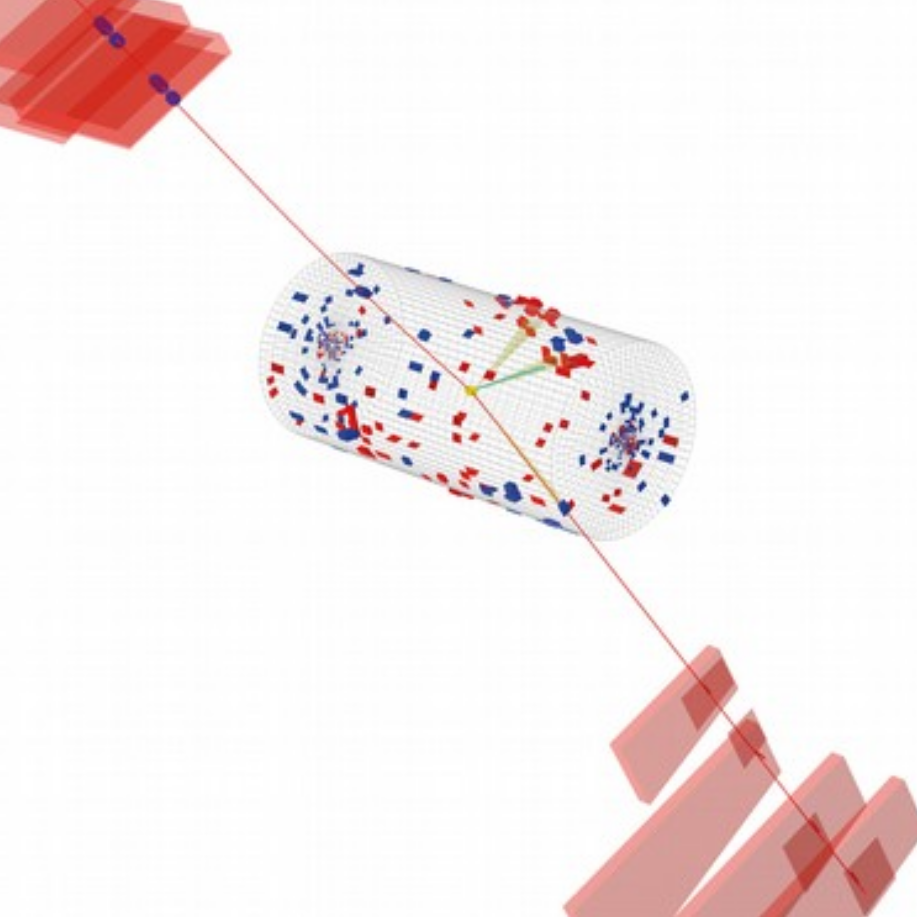
\includegraphics[width=\EmbedPictsWidth cm]{\PhDthesisdir/plots_and_images/from_embedding/Z_to_mumu_data.png}}};

\draw [-latex, very thick] (\EmbedPictsWidth+\EmbedPictsMarginX/5, \EmbedPictsWidth/2) -- + (3*\EmbedPictsMarginX/5,0);
\draw (\EmbedPictsWidth/2+\EmbedPictsWidth+\EmbedPictsMarginX, \EmbedPictsWidth) node [above] {\EmbedPictsTxtSize Supression de la paire $\mu\mu$};
\node[anchor=south west,inner sep=0] at (\EmbedPictsWidth+\EmbedPictsMarginX,0) {\frame{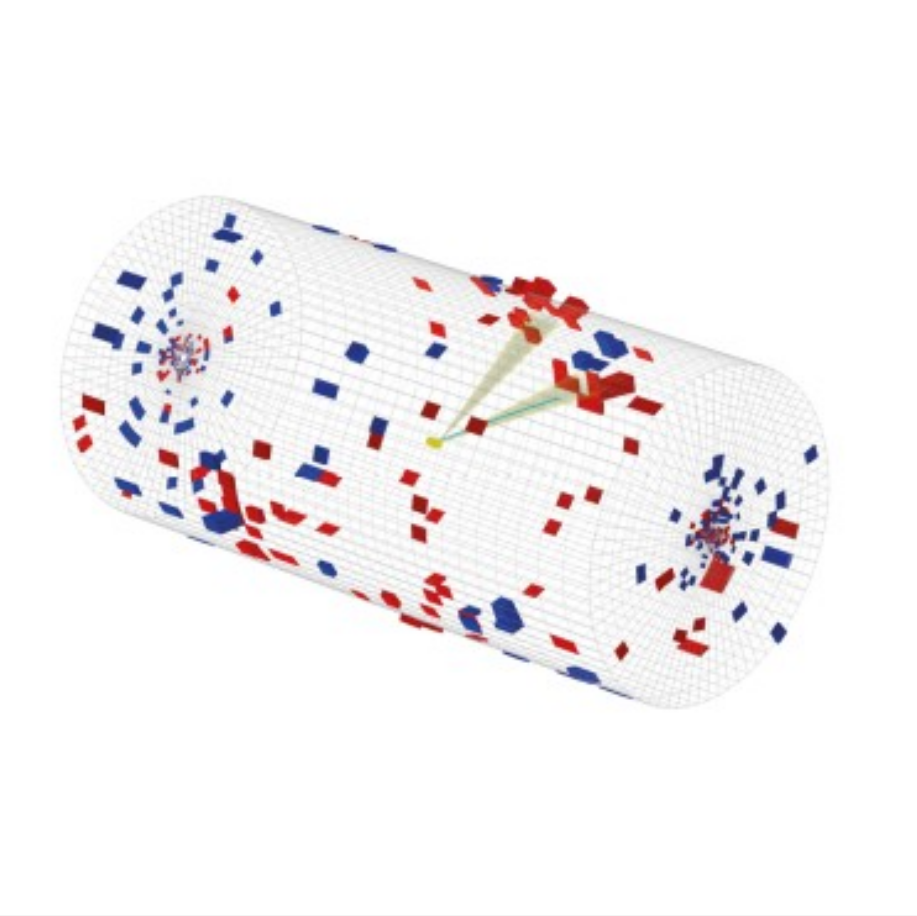
\includegraphics[width=\EmbedPictsWidth cm]{\PhDthesisdir/plots_and_images/from_embedding/remove_mumu.png}}};

\draw (\EmbedPictsWidth+\EmbedPictsMarginX,-\EmbedPictsWidth/2-\EmbedPictsMarginY) node [above left] {\EmbedPictsTxtSize Simulation des \tau};
\draw (\EmbedPictsWidth+\EmbedPictsMarginX,-\EmbedPictsWidth/2-\EmbedPictsMarginY) node [below left] {\EmbedPictsTxtSize ($\vec{p}_{\tau} \Leftrightarrow \vec{p}_{\mu}$)};
\node[anchor=south west,inner sep=0] at (\EmbedPictsWidth+\EmbedPictsMarginX,-\EmbedPictsWidth-\EmbedPictsMarginY) {\frame{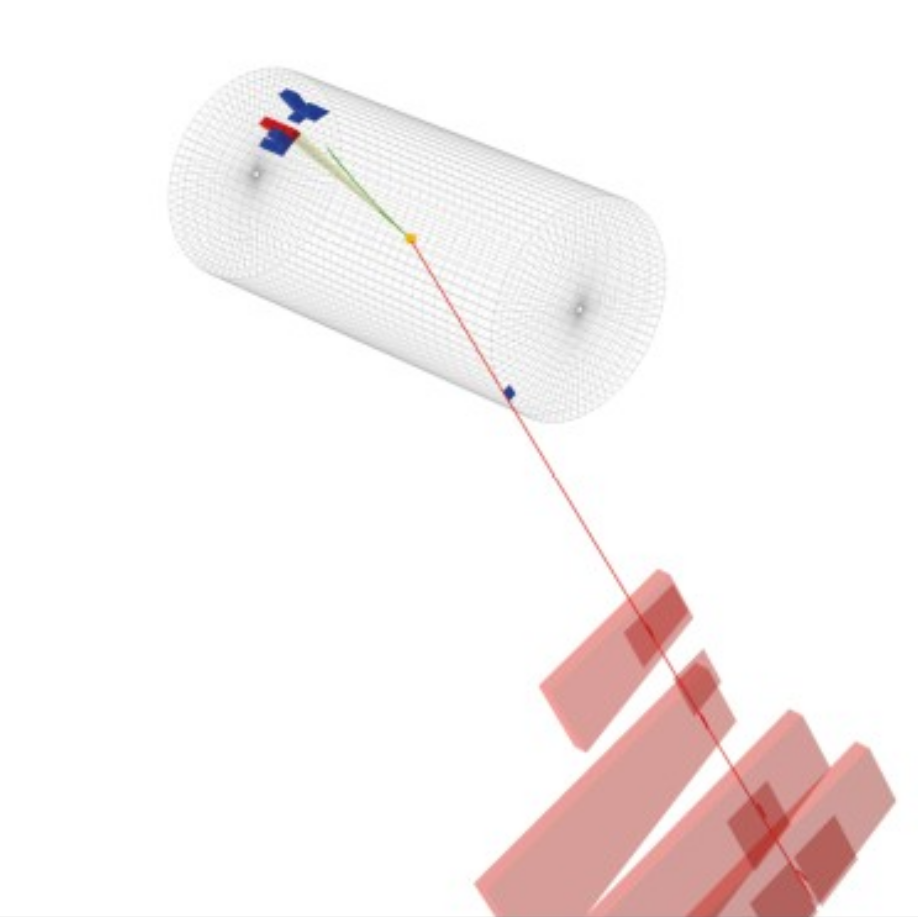
\includegraphics[width=\EmbedPictsWidth cm]{\PhDthesisdir/plots_and_images/from_embedding/Z_to_tautau_simulation.png}}};

\draw [-latex, very thick] (2*\EmbedPictsWidth+6*\EmbedPictsMarginX/5, \EmbedPictsWidth/4) -- (2*\EmbedPictsWidth+2*\EmbedPictsMarginX-\EmbedPictsMarginX/5,0);
\draw [-latex, very thick] (2*\EmbedPictsWidth+6*\EmbedPictsMarginX/5,-\EmbedPictsWidth/4-\EmbedPictsMarginY) -- (2*\EmbedPictsWidth+2*\EmbedPictsMarginX-\EmbedPictsMarginX/5,-\EmbedPictsMarginY);
\draw (2*\EmbedPictsWidth+2*\EmbedPictsMarginX+\EmbedPictsWidth/2,\EmbedPictsWidth/2-\EmbedPictsMarginY/2) node [above] {\EmbedPictsTxtSize Données encapsulées};
\node[anchor=south west,inner sep=0] at (2*\EmbedPictsWidth+2*\EmbedPictsMarginX,-\EmbedPictsWidth/2-\EmbedPictsMarginY/2) {\frame{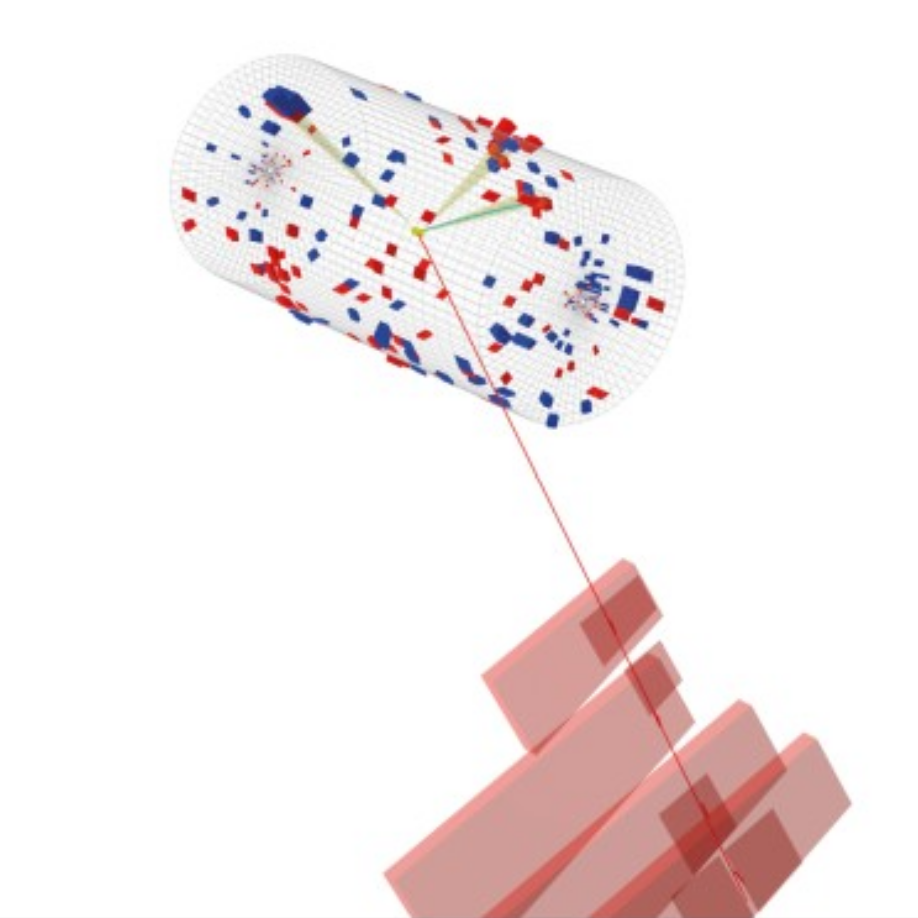
\includegraphics[width=\EmbedPictsWidth cm]{\PhDthesisdir/plots_and_images/from_embedding/embedded_event.png}}};

\clip (-1,-\EmbedPictsWidth-\EmbedPictsMarginY-.25) rectangle (3*\EmbedPictsWidth+5*\EmbedPictsMarginX/2+.25, \EmbedPictsWidth+.5);
\end{tikzpicture}
\caption[Schéma récapitulatif de la méthode des données encapsulées.]{Schéma récapitulatif de la méthode des données encapsulées~\cite{embedding}.}
\label{fig-embedding_recap}
\end{figure}
\par
Les données encapsulées nécessitent ainsi l'utilisation de simulation uniquement pour la paire de leptons taus et leurs désintégrations.
Tous les autres objets présents sont issus de données réelles.
L'empilement, l'événement sous-jacent et les jets de l'événement principal sont donc décrits de manière parfaitement identique à la réalité, dans la mesure où ils ne sont pas simulés.
De plus, l'incertitude sur la luminosité est supprimée pour les données encapsulées, car leur quantité est directement reliée à celle des données réelles, ce qui n'est pas le cas pour les données entièrement simulées.
Enfin, les effets dus au détecteur tels que le bruit inhérent à la mesure, les pièces défectueuses et son vieillissement sont naturellement inclus dans les données encapsulées.
\par
L'amélioration de la description des données ainsi obtenue grâce à l'encapsulement est visible sur la figure~\ref{fig-embedding_2018mt_puppimet_illustration}, où les distributions de l'énergie transverse manquante dans les données et dans l'estimation du bruit de fond sans et avec cette méthode sont tracées à titre d'illustration.
L'accord est sensiblement amélioré pour $\MET < \SI{30}{\GeV}$.
\begin{figure}[h]
\centering

\subcaptionbox{Sans l'encapsulement.}[.475\textwidth]
{\plotHTTcontrol{2018}{fully_classic}{mt}{puppimet}}
\hfill
\subcaptionbox{Avec l'encapsulement.}[.475\textwidth]
{\plotHTTcontrol{2018}{emb_classic}{mt}{puppimet}}

\caption{Distributions de \MET\ pour le canal \mu\tauh\ en 2018.}
\label{fig-embedding_2018mt_puppimet_illustration}
\end{figure}

\subsection{Méthode des facteurs de faux ou \emph{fake factors}}\label{chapter-HTT_analysis-section-bg_estimation-FF_method}
La méthode des facteurs de faux (\emph{fake factors}) a pour but de fournir, en se basant presque exclusivement sur les données collectées, une estimation des bruits de fond dans lesquels des jets, provenant de quarks ou de gluons, sont identifiés à tort comme des taus hadroniques (\tauh).
De tels jets sont notés \og \ftauh \fg{} dans la suite.
\par
Cette méthode est ainsi appliquée aux canaux contenant des \tauh\ dans l'état final, \ie\ les canaux complètement hadronique (\tauh\tauh) et semi-leptoniques ($\ell\tauh$ où $\ell\in\set{\ele,\mu}$).
Les \ftauhs\ représentent près de \SI{70}{\%} des événements dans le canal \tauh\tauh, \SI{38}{\%} dans le canal \mu\tauh\ et \SI{68}{\%} dans le canal \ele\tauh~\cite{CMS-NOTE-2018-257,CMS-NOTE-2019-170}.
Les processus physiques responsables des \ftauhs\ sont majoritairement QCD, \Wjets\ et \ttbar.
Dans le canal \tauh\tauh, près de \SI{93}{\%} des \ftauhs\ proviennent du bruit de fond QCD.
Dans les canaux $\ell\tauh$, environ \SI{70}{\%} des \ftauhs\ sont issus du bruit de fond \Wjets.
Les autres sources de \ftauhs, non traités par cette méthode, sont les événements $\Zboson\to\tau\tau$ avec un jet identifié comme un \tauh, couverts par la méthode décrite section~\ref{chapter-HTT_analysis-section-bg_estimation-embedding}, et Diboson, ce dernier type de processus ne contribuant que de l'ordre du pourcent au total des \ftauhs.
\par
Les \ftauhs\ sont particulièrement difficiles à modéliser dans les simulations~\cite{CMS-NOTE-2018-257,CMS-NOTE-2019-170}.
De plus, le faible de taux de mauvaise identification des \tauh, inférieur à \SI{1}{\%}, impliquerait l'utilisation de larges jeux de données simulées afin d'obtenir de faibles incertitudes statistiques.
C'est en particulier le cas dans les régions de l'espace des phases contenant des bosons de Higgs lourds, ce que recherche cette analyse.
La méthode des \fakefactors\ se basant presque exclusivement sur les données collectées, les incertitudes inhérentes aux simulations deviennent négligeables face aux autres sources d'incertitudes.
De plus, l'efficacité statistique de cette modélisation est directement liée à la luminosité intégrée, sans nécessiter de données simulées correspondantes.
\subsubsection{Principe de base}
Cette méthode suit le même principe de produit en croix que la méthode \og ABCD \fg{} présentée section~\ref{chapter-HTT_analysis-section-bg_estimation-QCD-SS} mais va plus loin dans la détermination du facteur $C/D$ nommé ici \fakefactor.
Dans une région de contrôle, détaillée dans la section suivante, le rapport des quantités de \tauh\ isolés sur ceux anti-isolés est déterminé.
Il s'agit du \fakefactor\, noté \FF, défini comme
\begin{equation}
\FF = \frac{n_\text{iso}}{n_\text{anti-iso}} = \frac{n(\texttt{Medium})}{n(\texttt{VVVLoose \&\& !Medium})}
\label{eq-chapter-HTT_analysis-section-bg_estimation-FF_method-FF_def_global}
\end{equation}
où
\begin{itemize}
\item $n(\texttt{Medium})$ est la quantité d'événements dans la région de contrôle (CR, \emph{Control Region}) passant le point de fonctionnement \PassDeepTau{moyen}{medium}{vs jet}, utilisé également pour sélectionner les événements de signal;
\item $n(\texttt{VVVLoose \&\& !Medium})$ est la quantité d'événements dans la région de contrôle passant le point de fonctionnement le plus lâche de ce discriminateur, mais pas le moyen.
\end{itemize}
Le \fakefactor\ \FF\ est déterminé de manière indépendante pour chaque canal (\tauh\tauh, \mu\tauh, \ele\tauh), chaque année (2016, 2017, 2018) et dépend:
\begin{itemize}
\item de l'impulsion transverse de l'objet physique identifié comme un \tauh, $\pT^{\tauh}$;
\item de l'impulsion transverse du jet le plus proche du \tauh, $\pT^\text{jet}$;
\item du nombre de jets tels que $\abs{\eta^\text{jet}}<\num{2.4}$ et $\pT^\text{jet}>\SI{20}{\GeV}$, \Nprebjets.
\end{itemize}
\par
Une région d'application du \fakefactor\ (AR, \emph{Application Region}) est définie de manière similaire à la région de signal (SR, \emph{Signal Region}), seul le critère d'isolation des \tauh\ passe de \og isolé \fg{}  à \og anti-isolé \fg.
La AR est ainsi riche en \ftauhs.
La quantité d'événements contenant des \ftauhs\ dans la SR, notée $n_{j\to\tauh}$, est alors obtenue par produit en croix avec la quantité d'événements dans la AR, notée $n_\text{AR}$,  selon
\begin{equation}
n_{j\to\tauh} = n_\text{AR} \cdot \FF
\mend[,]
\end{equation}
l'hypothèse étant l'universalité, \ie\ que le \fakefactor\ mesuré dans la CR est supposé identique à celui de la AR.
\subsubsection{Prise en compte des différentes sources de \ftauhs}
La composition des jets n'est pas la même selon le processus physique dont proviennent les \ftauhs.
Il existe donc différentes probabilités pour un jet de donner un \ftauh.
Dans le cas du canal \tauh\tauh, seul le bruit de fond QCD est traité par les \fakefactors.
Pour les canaux semi-leptoniques, trois sources de \ftauhs\ sont considérées, QCD, \Wjets\ et \ttbar.
Pour chacune de ces sources, un \fakefactor\ est alors déterminé, selon l'équation~\eqref{eq-chapter-HTT_analysis-section-bg_estimation-FF_method-FF_def_global}, à partir d'une région de détermination (DR, \emph{Determination Region}) dédiée, définie ci-après.
Du fait de la séparation de la CR en plusieurs DR, l'universalité n'est alors plus complètement garantie.
Des corrections résiduelles sont appliquées afin de corriger le biais introduit par la séparation en DR.
\par
Le \fakefactor\ global est ainsi la moyenne des \fakefactors\ obtenus pour chaque source, avec comme coefficients les fractions $f$ d'événements de ces sources dans la AR, \ie
\begin{equation}
\FF = \sum_i f_i \cdot \FF_i
\msep
f_i = \frac{n_\text{AR}^i}{\sum_j n_\text{AR}^{j}}
\msep
i,j \in \set{\text{QCD, \Wjets, \ttbar}}
\mend
\end{equation}
Les fractions $f_i$ sont déterminées à partir de simulations et dépendent:
\begin{itemize}
\item de la masse transverse du lepton $\ell\in\set{\ele,\mu}$, $\mT^{\ell}$;
\item du nombre de jets \Nprebjets\ identifiés comme issus de quarks~\quarkb, \Nbjets;
\item de la masse transverse totale, définie équation~\eqref{eq-def_mTtot}, \mTtot.
\end{itemize}
La figure~\ref{fig-chapter-HTT_analysis-section-bg_estimation-FF_method-fractions} présente ces fractions en fonction de \mTtot\ pour $\mT^{\mu} < \SI{40}{\GeV}$ et $\Nbjets\in\set{0,\geq1}$ pour le canal \mu\tauh\ en 2018.
La méthode des \fakefactors\ est résumée figure~\ref{fig-chapter-HTT_analysis-section-bg_estimation-FF_method-ppe}.
\begin{figure}[h]
\centering

\subcaptionbox{Pour $\Nbjets=0$ et $\mT^{\mu} < \SI{40}{\GeV}$}[.45\textwidth]
{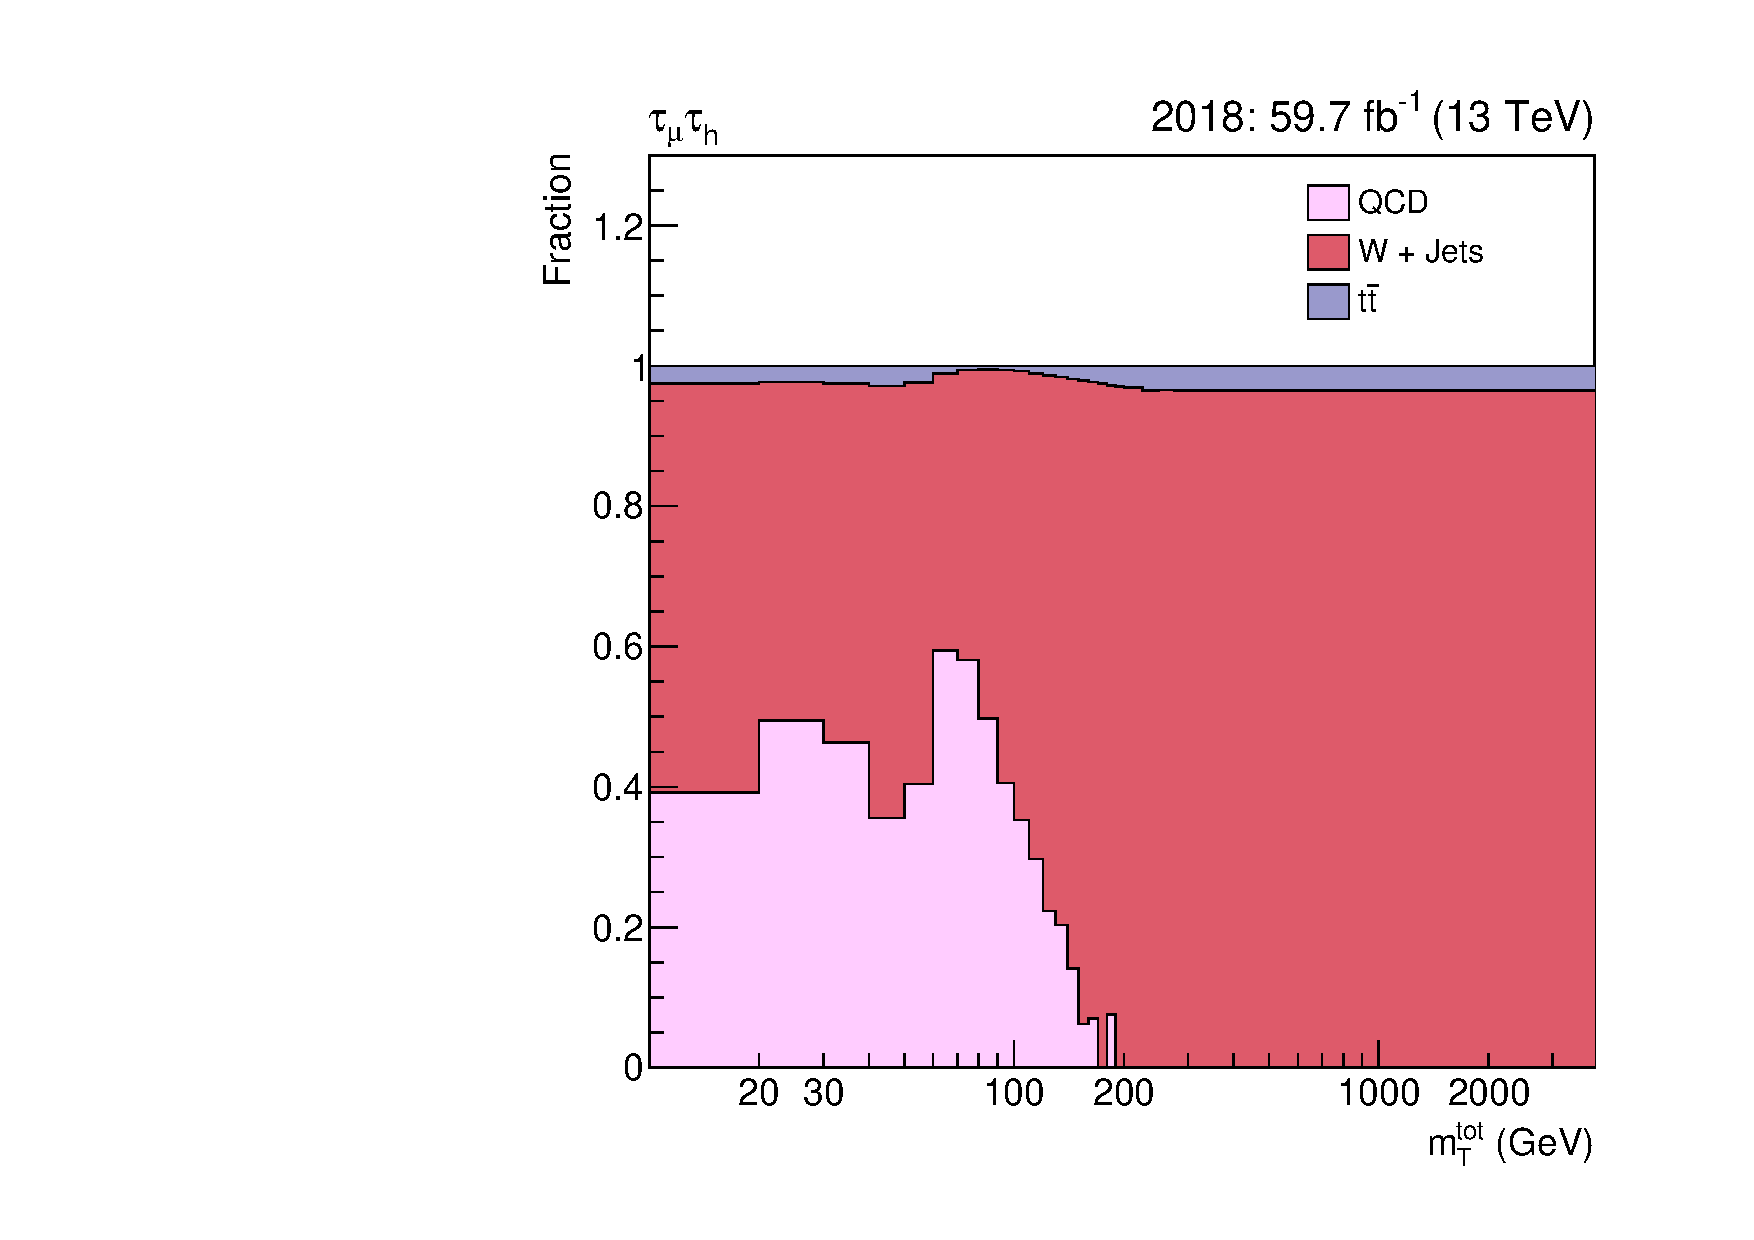
\includegraphics[width=.45\textwidth]{\PhDthesisdir/plots_and_images/from_CMS-NOTE-2020-218/ff_fraction_tightmt_nbjets0_mt_2018_os_rebinning.tex}}
\hfill
\subcaptionbox{Pour $\Nbjets\geq1$ et $\mT^{\mu} < \SI{40}{\GeV}$}[.45\textwidth]
{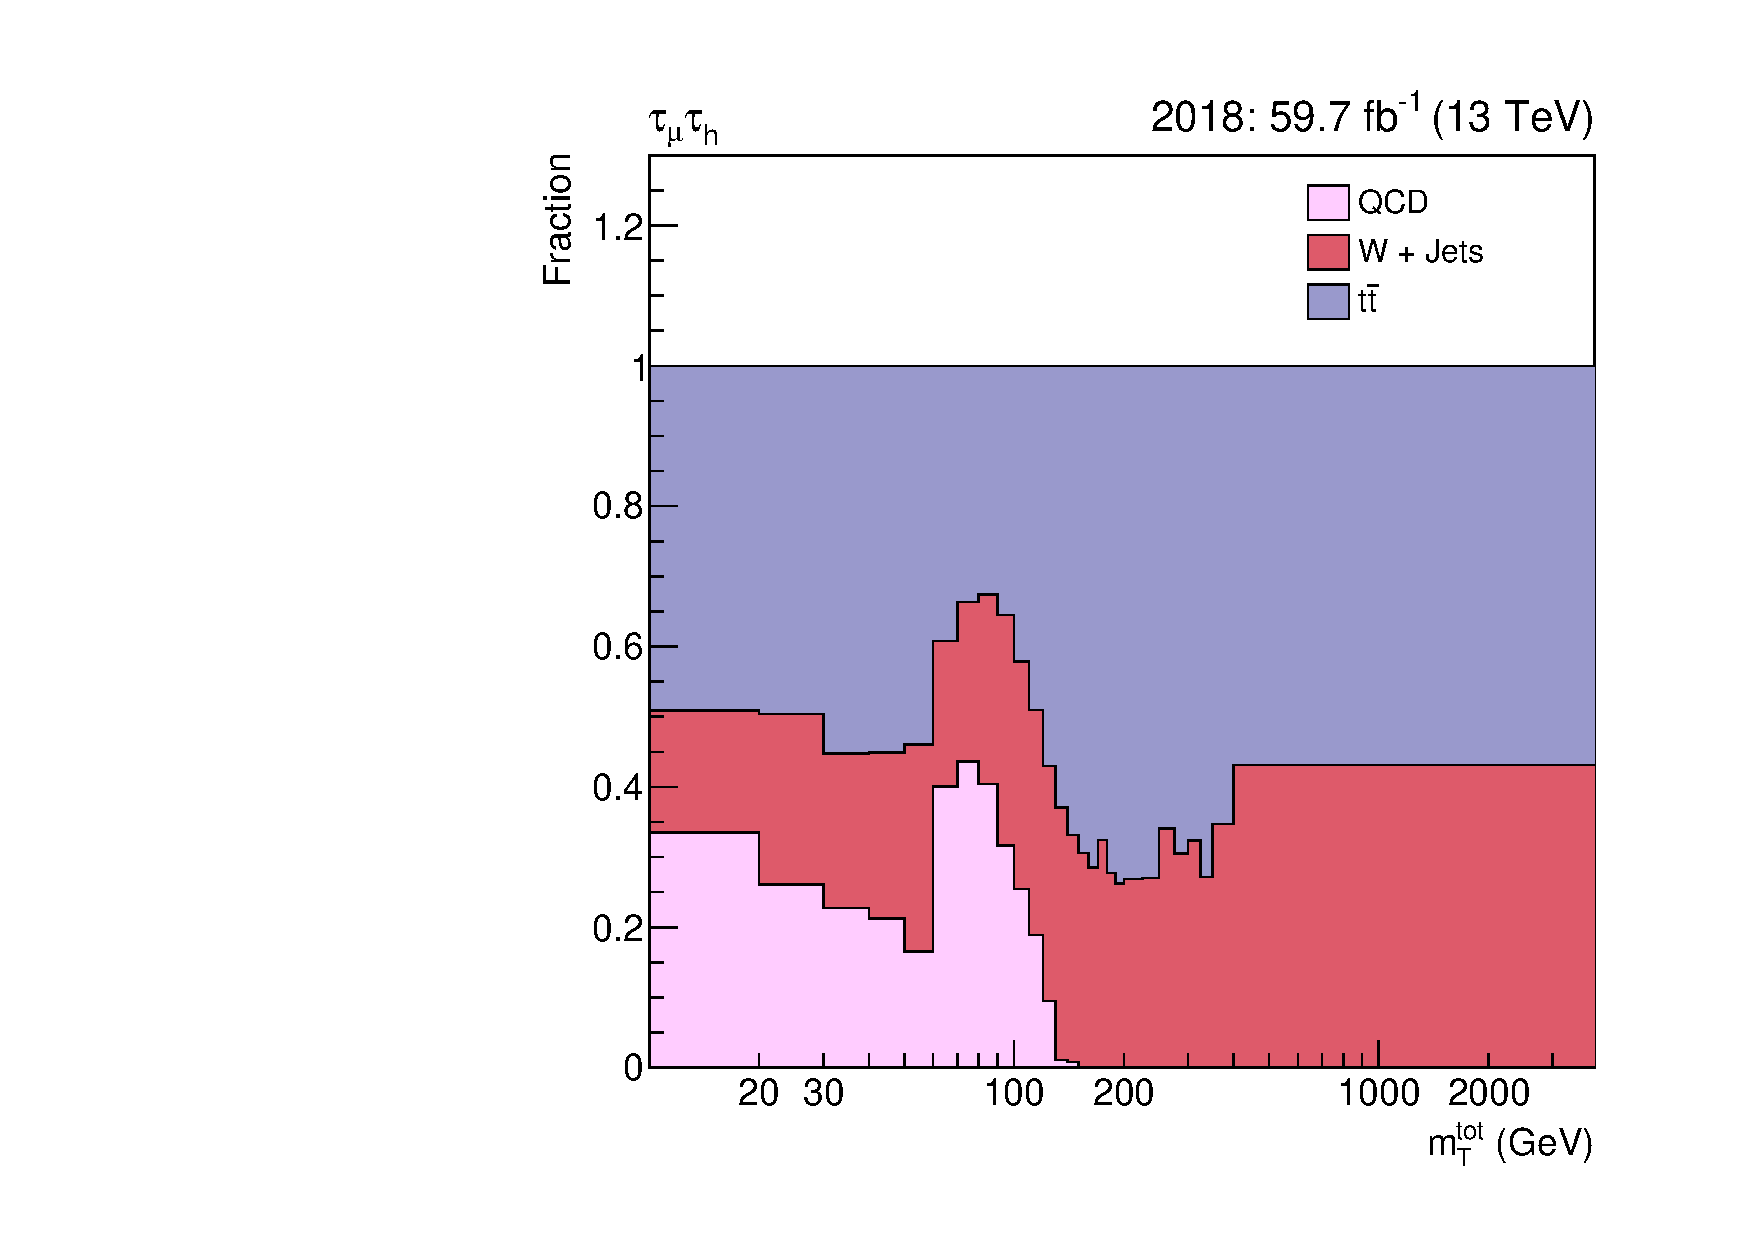
\includegraphics[width=.45\textwidth]{\PhDthesisdir/plots_and_images/from_CMS-NOTE-2020-218/ff_fraction_tightmt_nbjets1_mt_2018_os_rebinning.tex}}

\caption[Fractions des sources de \ftauhs\ dans le canal \mu\tauh\ en 2018.]{Fractions des sources de \ftauhs\ dans le canal \mu\tauh\ en 2018~\cite{CMS-NOTE-2020-218}.}
\label{fig-chapter-HTT_analysis-section-bg_estimation-FF_method-fractions}
\end{figure}
\begin{figure}[h]
\centering
\begin{tikzpicture}
\def\RegionW{3}
\def\RegionH{2.5}

\fill [ltcolorgray2] (0,0) rectangle + (\RegionW,\RegionH);
\fill [ltcolorred2] (\RegionW,0) rectangle + (\RegionW,\RegionH);
\fill [ltcolormagenta2] (2*\RegionW,0) rectangle + (\RegionW,\RegionH);
\fill [ltcolorviolet2] (3*\RegionW,0) rectangle + (\RegionW,\RegionH);

\fill [ltcolorgray1] (0,\RegionH) rectangle + (\RegionW,\RegionH);
\fill [ltcolorred1] (\RegionW,\RegionH) rectangle + (\RegionW,\RegionH);
\fill [ltcolormagenta1] (2*\RegionW,\RegionH) rectangle + (\RegionW,\RegionH);
\fill [ltcolorviolet1] (3*\RegionW,\RegionH) rectangle + (\RegionW,\RegionH);

\draw [ultra thick, -latex] (0.875*\RegionW, \RegionH-\RegionW/6) --+ (0,\RegionW/3);

%\draw (1.5*\RegionW, \RegionH) node [above] (FFW) {\Large $\FF_\Wboson$};
%\draw (2.5*\RegionW, \RegionH) node [above] (FFQ) {\Large $\FF_Q$};
%\draw (3.5*\RegionW, \RegionH) node [above] (FFT) {\Large $\FF_\quarkt$};

\foreach \value/\DeterminationRegion/\nodecoord in {1.5/\Wboson/FFW, 2.5/Q/FFQ, 3.5/\quarkt/FFT}{
\draw (\value*\RegionW, \RegionH) node (\nodecoord) {\large $\displaystyle \FF_{\DeterminationRegion}=\frac{n_\text{iso}^{\DeterminationRegion}}{n_\text{anti-iso}^{\DeterminationRegion}}$};
}

\draw [ultra thick] (1*\RegionW,1.4*\RegionH)  to [out=0,in=90, out looseness = 1.5, in looseness = 1] (5*\RegionW/4,8*\RegionH/7);
\draw [ultra thick] (2*\RegionW,1.4*\RegionH)  to [out=0,in=90, out looseness = 1.5, in looseness = 1] (9*\RegionW/4,8*\RegionH/7);

\draw [ultra thick, latex-] (.9*\RegionW,1.4*\RegionH) -- (3*\RegionW,1.4*\RegionH)  to [out=0,in=90, out looseness = 1.5, in looseness = 1] (13*\RegionW/4,8*\RegionH/7);

\draw [thick, -latex] (-\RegionW/5,0) -- (4*\RegionW,0) --+ (\RegionW/5,0) node [right] {Région};
\draw [thick, -latex] (0,-\RegionW/5) -- (0,2*\RegionH) --+ (0,\RegionW/5) node [above] {Isolation du \tauh};

\draw (-0*\RegionW, 1.5*\RegionH) node [above, rotate=90] {isolé};

\draw (-0*\RegionW, .5*\RegionH) node [above, rotate=90] {anti-isolé};

\draw (.45*\RegionW, .675*\RegionH) node {\small fractions des};
\draw (.45*\RegionW, .525*\RegionH) node {\small processus};
\draw (\RegionW, .6*\RegionH) node [left] {$\mathrm{f}_i$};

\draw (.45*\RegionW, .275*\RegionH) node {\small quantité};
\draw (.45*\RegionW, .125*\RegionH) node {\small d'événements};
\draw (\RegionW, .2*\RegionH) node [left] {$n_\text{AR}$};


\draw (.5*\RegionW, 1.65*\RegionH) node {$n_\text{AR}\cdot\sum_i f_i \cdot \FF_i$\ };
\draw (.5*\RegionW, 1.4*\RegionH) node {$=n_{j\to\tauh}$};

\draw (.5*\RegionW, 2*\RegionH) node [below] {\textbf{SR}};
\draw (.5*\RegionW, 1*\RegionH) node [below] {\textbf{AR}};

% $\Wboson+\text{jets}$, QCD multijet, $\ttbar+\text{jets}$

\draw (0.5*\RegionW, 0) node [below] {AR \& SR} ;
\draw (1.5*\RegionW, 0) node [below] {DR \Wjets} ;
\draw (2.5*\RegionW, 0) node [below] {DR QCD} ;
\draw (3.5*\RegionW, 0) node [below] {DR \ttbar} ;

\end{tikzpicture}
\caption[Illustration de la méthode des \fakefactors.]{Illustration de la méthode des \fakefactors. Les \fakefactors\ sont obtenus à partir du nombre d'événements avec des \tauh\ isolés et anti-isolés dans les régions de détermination (DR) de chaque processus contribuant significativement au bruit de fond contenant des \ftauhs. La quantité de \ftauhs\ dans la région de signal (SR) est estimée à partir des fractions de ces processus et du nombre d'événements présents dans la région d'application (AR).}
\label{fig-chapter-HTT_analysis-section-bg_estimation-FF_method-ppe}
\end{figure}
\subsubsection{Régions de détermination}
\paragraph{QCD}
La DR QCD est définie de la même manière que la SR à l'exception du critère sur les charges électriques des éléments du \emph{dilepton}.
En effet, ceux-ci doivent être de charges opposées (OS, \emph{Opposite Signs}) dans la SR car les bosons de Higgs recherchés étant neutres, la charge globale du \emph{dilepton} doit, par conservation, être nulle.
Pour la DR QCD, ces charges doivent être de même signe (SS, \emph{Same Sign}).
Dans le cas des canaux $\ell\tauh$, il est de plus requis que $I_\text{rel}^{\ell} > \num{0.05}$ afin de réduire les contribution de processus donnant des électrons ou des muons sans objet physique pertinent pour les \fakefactors.
Les contributions d'autres processus à la DR est soustraite grâce à l'utilisation de données simulées.
Pour le canal \tauh\tauh, le \fakefactor\ $\FF_Q$ est déterminé uniquement pour le premier \tauh\ (de plus haut \pT).
\par
Le \fakefactor\ $\FF_Q$ est mesuré séparément pour:
\begin{itemize}
\item $\Nprebjets=0$;
\item $\Nprebjets\geq1$;
\end{itemize}
et dans chacun de ces deux cas pour
\begin{itemize}
\item $\pT^\text{jet}/\pT^{\tauh} < \num{1.25}$;
\item $\num{1.25} \leq \pT^\text{jet}/\pT^{\tauh} < \num{1.5}$;
\item $\num{1.5} \leq \pT^\text{jet}/\pT^{\tauh}$.
\end{itemize}
Pour ces six catégories, la dépendance en $\pT^{\tauh}$ de $\FF_Q$ est modélisée polynôme de degré 3 ajusté aux mesures pour $\pT^{\tauh}<\SI{200}{\GeV}$.
\par
Dans le cas du canal \tauh\tauh, peu d'événements sont disponibles pour $\pT^{\tauh}\geq\SI{200}{\GeV}$.
Le \fakefactor\ $\FF_Q$ est ainsi fixé à la valeur mesurée pour $\pT^\text{jet}/\pT^{\tauh} \geq \num{1.5}$ et à la valeur à \SI{200}{\GeV} du polynôme pour $\pT^\text{jet}/\pT^{\tauh} < \num{1.5}$.
Pour les canaux $\ell\tauh$, la situation est similaire à partir de $\pT^{\tauh}\geq\SI{140}{\GeV}$.
La valeur utilisée à haut $\pT^{\tauh}$ suit la logique suivante:
\begin{itemize}
\item si l'erreur relative sur $\FF_Q$ pour $\pT^{\tauh}\geq\SI{200}{\GeV}$ est inférieure à \num{0.5}:
\begin{itemize}
\item si l'erreur relative sur $\FF_Q$ pour $\pT^{\tauh}\in[140, 200]\usp\SI{}{\GeV}$ est inférieure à \num{0.5}, les valeurs mesurées sont utilisées sur les intervalles $[140, 200]\usp\SI{}{\GeV}$ et $[200, \infty[\usp\SI{}{\GeV}$,
\item si l'erreur relative sur $\FF_Q$ pour $\pT^{\tauh}\in[140, 200]\usp\SI{}{\GeV}$ est supérieure à \num{0.5}, la valeur mesurée est utilisée sur l'intervalle $[200, \infty[\usp\SI{}{\GeV}$;
\end{itemize}
\item si l'erreur relative sur $\FF_Q$ pour $\pT^{\tauh}\geq\SI{200}{\GeV}$ est supérieure à \num{0.5}
et inférieure à \num{0.5} pour $\pT^{\tauh}\in[140, 200]\usp\SI{}{\GeV}$,
la valeur mesurée est utilisée sur l'intervalle $[140, \infty[\usp\SI{}{\GeV}$;
\item sinon, la valeur obtenue par l'ajustement est utilisée.
\end{itemize}
%L'ajustement obtenu pour $\FF_Q$ sur le canal \mu\tauh\ en 2018 est illustré figure~\ref{fig-chapter-HTT_analysis-section-bg_estimation-FF_method-FFQ_fit} pour $\Nprebjets=0$ et $\num{1.5} \leq \pT^\text{jet}/\pT^{\tauh}$.
%\begin{figure}[h]
%\centering
%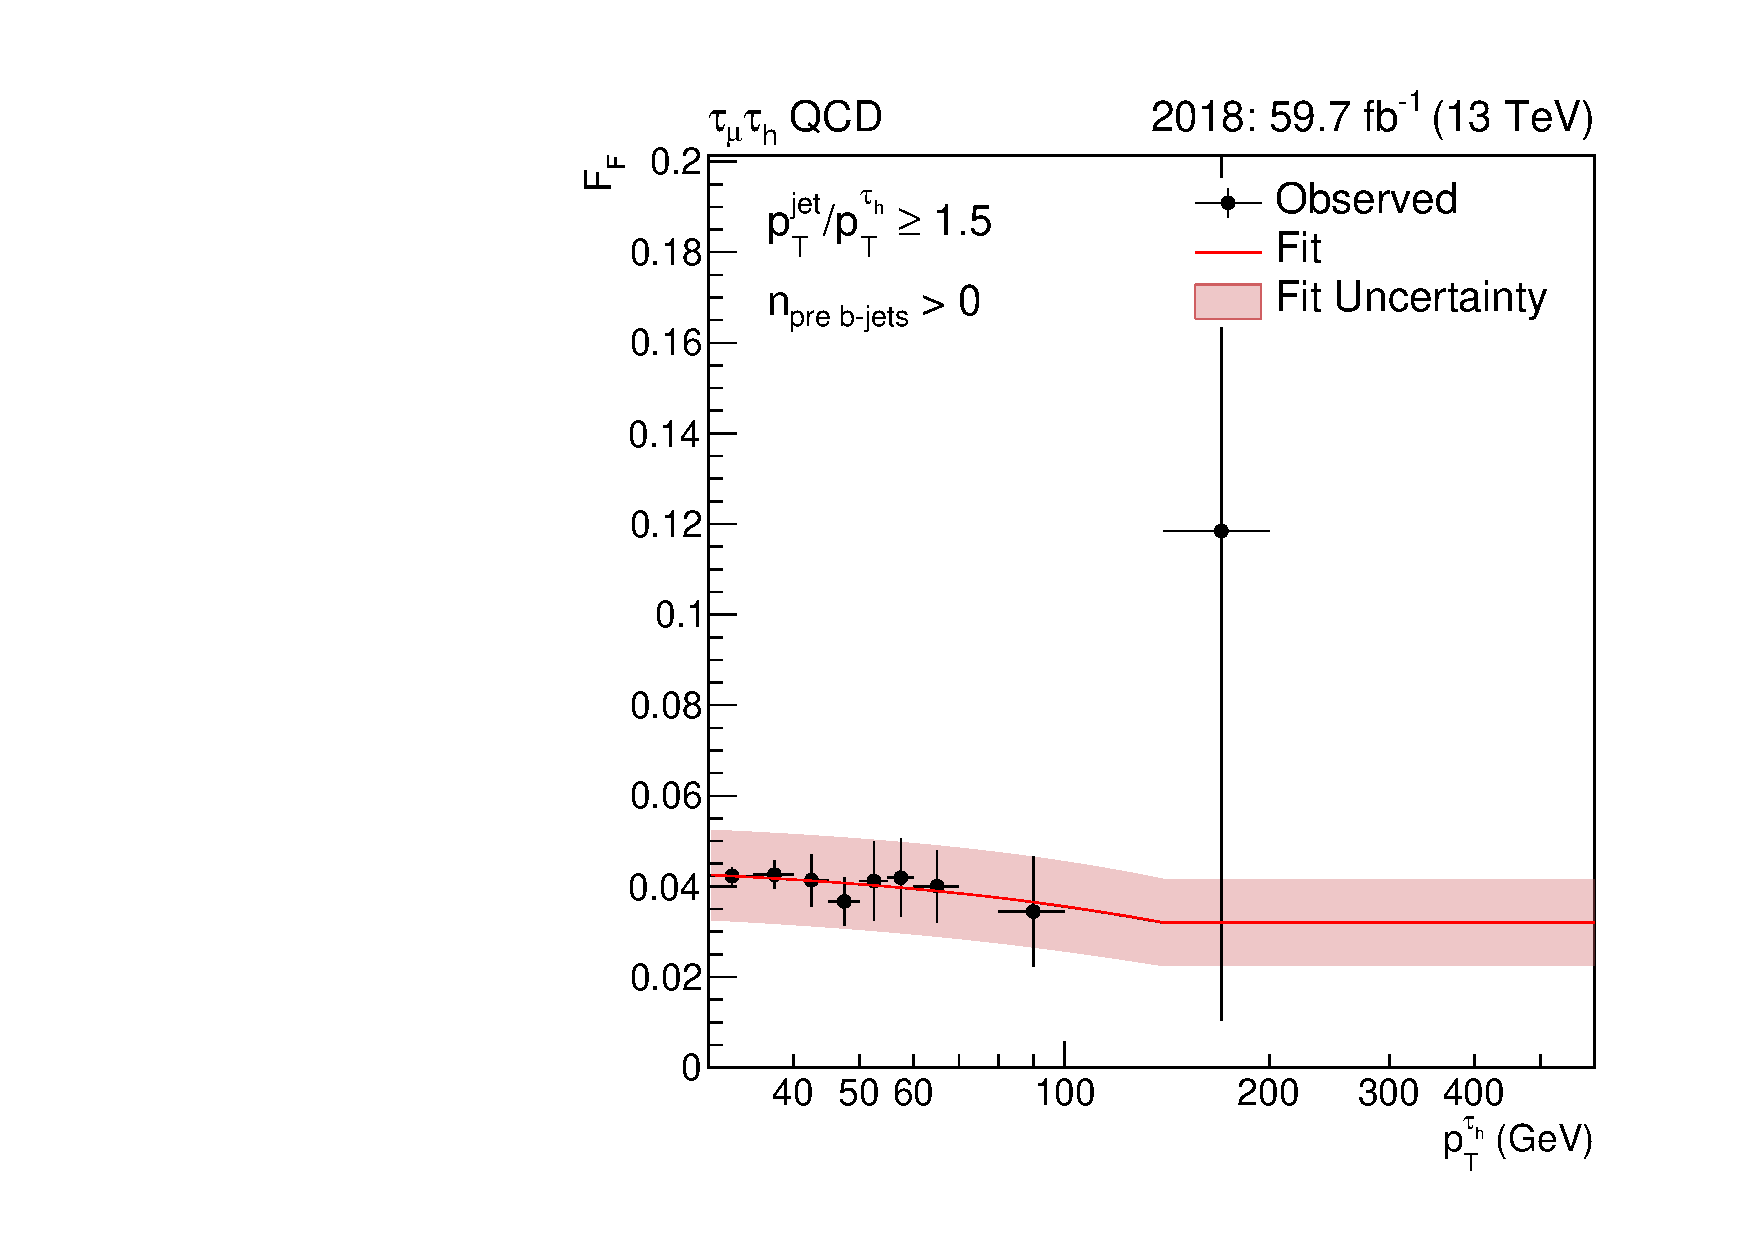
\includegraphics[width=.45\textwidth]{\PhDthesisdir/plots_and_images/from_CMS-NOTE-2020-218/ff_fit_jet_pt_high_1jet_pt_2_ff_qcd_mt_2018.tex}
%\caption[Ajustement de $\FF_Q$ dans le canal \mu\tauh\ en 2018.]{Ajustement de $\FF_Q$ dans le canal \mu\tauh\ en 2018~\cite{CMS-NOTE-2020-218}.}
%\label{fig-chapter-HTT_analysis-section-bg_estimation-FF_method-FFQ_fit}
%\end{figure}
\paragraph{\Wjets}
La DR \Wjets\ ne concerne que les canaux semi-leptoniques.
Elle est définie de la même manière que la SR à l'exception de la coupure sur la masse transverse du lepton qui doit ici être supérieure à \SI{70}{\GeV}, alors qu'elle est inférieure à cette même valeur dans la SR.
Il est de plus requis que $\Nbjets=0$ afin de supprimer la contamination par les événements \ttbar.
Les contributions d'autres processus physiques à la DR sont soustraites par l'utilisation directe de données simulées.
Le bruit de fond QCD à retirer est obtenu à partir des données réelles avec les charges électriques des éléments du \emph{dilepton} de même signe, auxquelles sont soustraites les autres bruits de fond avec charges électriques de même signe, y compris \Wjets, obtenus par simulation directe.
Un facteur correctif de \num{1.1} est appliqué aux données à retirer, correspondant au rapport observé d'événements avec charges opposées sur événements avec charges de même signe.
\par
Le \fakefactor\ $\FF_W$ est mesuré séparément pour:
\begin{itemize}
\item $\Nprebjets=0$;
\item $\Nprebjets\geq1$;
\end{itemize}
et dans chacun de ces deux cas pour
\begin{itemize}
\item $\pT^{\text{jet})}/\pT^{\tauh} < \num{1.25}$;
\item $\num{1.25} \leq \pT^\text{jet}/\pT^{\tauh} < \num{1.5}$;
\item $\num{1.5} \leq \pT^\text{jet}/\pT^{\tauh}$.
\end{itemize}
Pour ces six catégories, la dépendance en $\pT^{\tauh}$ de $\FF_Q$ est modélisée polynôme de degré 3 ajusté aux mesures pour $\pT^{\tauh}<\SI{140}{\GeV}$.
\par
Dans cette DR également, peu d'événements sont disponibles pour $\pT^{\tauh}\geq\SI{140}{\GeV}$.
La même logique que pour $\FF_Q$, détaillée précédemment, est suivie sur la valeur de $\FF_W$ à utiliser.
L'ajustement obtenu pour $\FF_W$ sur le canal \mu\tauh\ en 2018 est illustré figure~\ref{subfig-chapter-HTT_analysis-section-bg_estimation-FF_method-WJ} pour $\Nprebjets\geq1$ et $\num{1.25} \leq \pT^\text{jet}/\pT^{\tauh} < \num{1.5}$.
Il y apparaît l'effet du traitement de la région à haut $\pT^{\tauh}$.
\paragraph{\ttbar}
La DR \ttbar\ ne concerne que les canaux semi-leptoniques.
Il n'est pas possible de définir une DR issue des données suffisamment pure pour mesurer $\FF_t$.
Ce \fakefactor\ est alors obtenu à partir de données simulées.
\par
Le \fakefactor\ $\FF_W$ peut également être mesuré à partir de données simulées uniquement.
Un écart de \num{10} à \SI{20}{\%} avec le \fakefactor\ obtenu à partir des données réelles est observé.
La contribution \ttbar\ étant faible par rapport aux autres bruits de fond rend négligeable le biais introduit par l'utilisation de données simulées face aux incertitudes sur les \fakefactors.
\par
Le \fakefactor\ $\FF_t$ est mesuré séparément pour:
\begin{itemize}
\item $\pT^\text{jet}/\pT^{\tauh} < \num{1.25}$;
\item $\num{1.25} \leq \pT^\text{jet}/\pT^{\tauh} < \num{1.5}$;
\item $\num{1.5} \leq \pT^\text{jet}/\pT^{\tauh}$;
\end{itemize}
sans séparation en \Nprebjets, la majorité des événements \ttbar\ vérifiant $\Nprebjets\geq1$.
L'ajustement obtenu pour $\FF_t$ sur le canal \mu\tauh\ en 2018 est illustré figure~\ref{subfig-chapter-HTT_analysis-section-bg_estimation-FF_method-ttbar} pour $\pT^\text{jet}/\pT^{\tauh} < \num{1.25}$.
\begin{figure}[h]
\centering

\subcaptionbox{Ajustement de $\FF_W$.\label{subfig-chapter-HTT_analysis-section-bg_estimation-FF_method-WJ}}[.45\textwidth]
{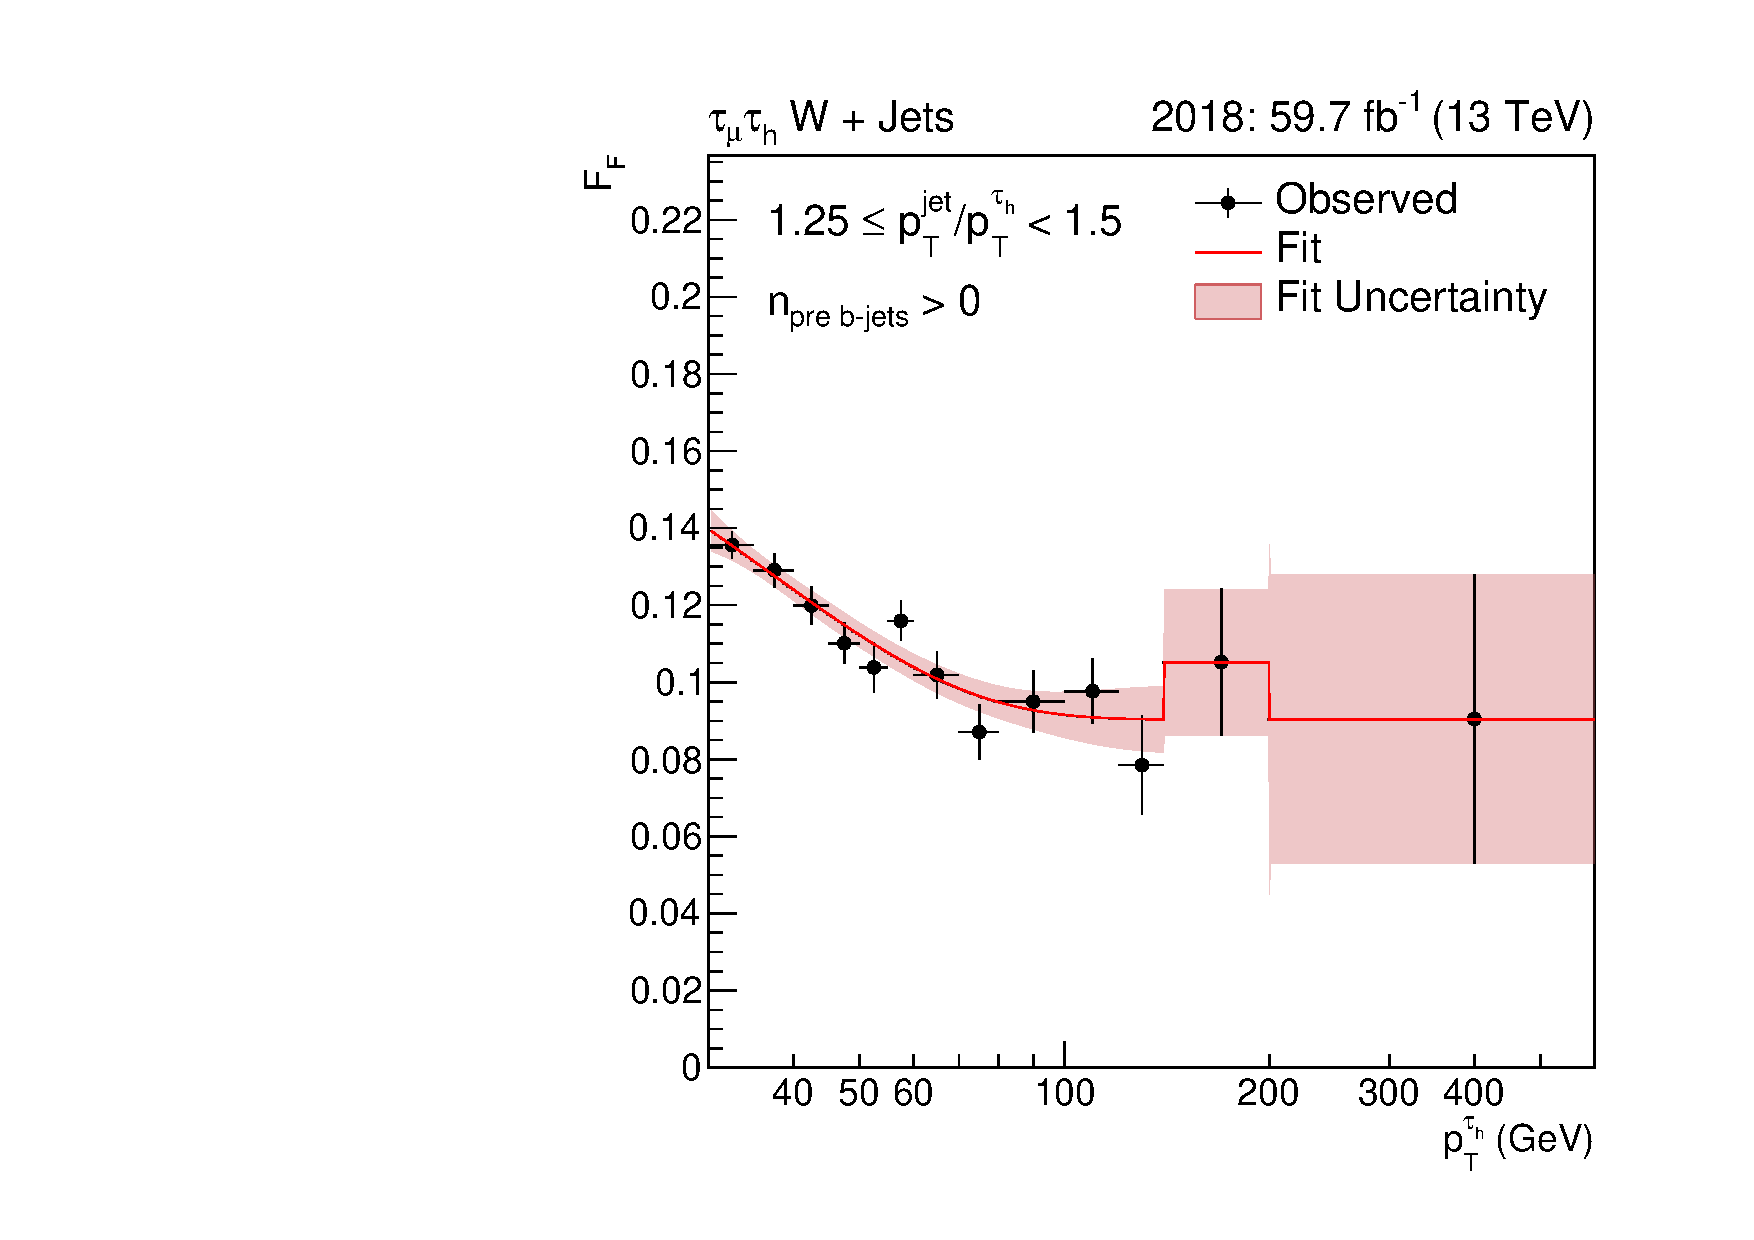
\includegraphics[width=.45\textwidth]{\PhDthesisdir/plots_and_images/from_CMS-NOTE-2020-218/ff_fit_jet_pt_med_1jet_pt_2_ff_wjets_mt_2018.tex}}
\hfill
\subcaptionbox{Ajustement de $\FF_t$.\label{subfig-chapter-HTT_analysis-section-bg_estimation-FF_method-ttbar}}[.45\textwidth]
{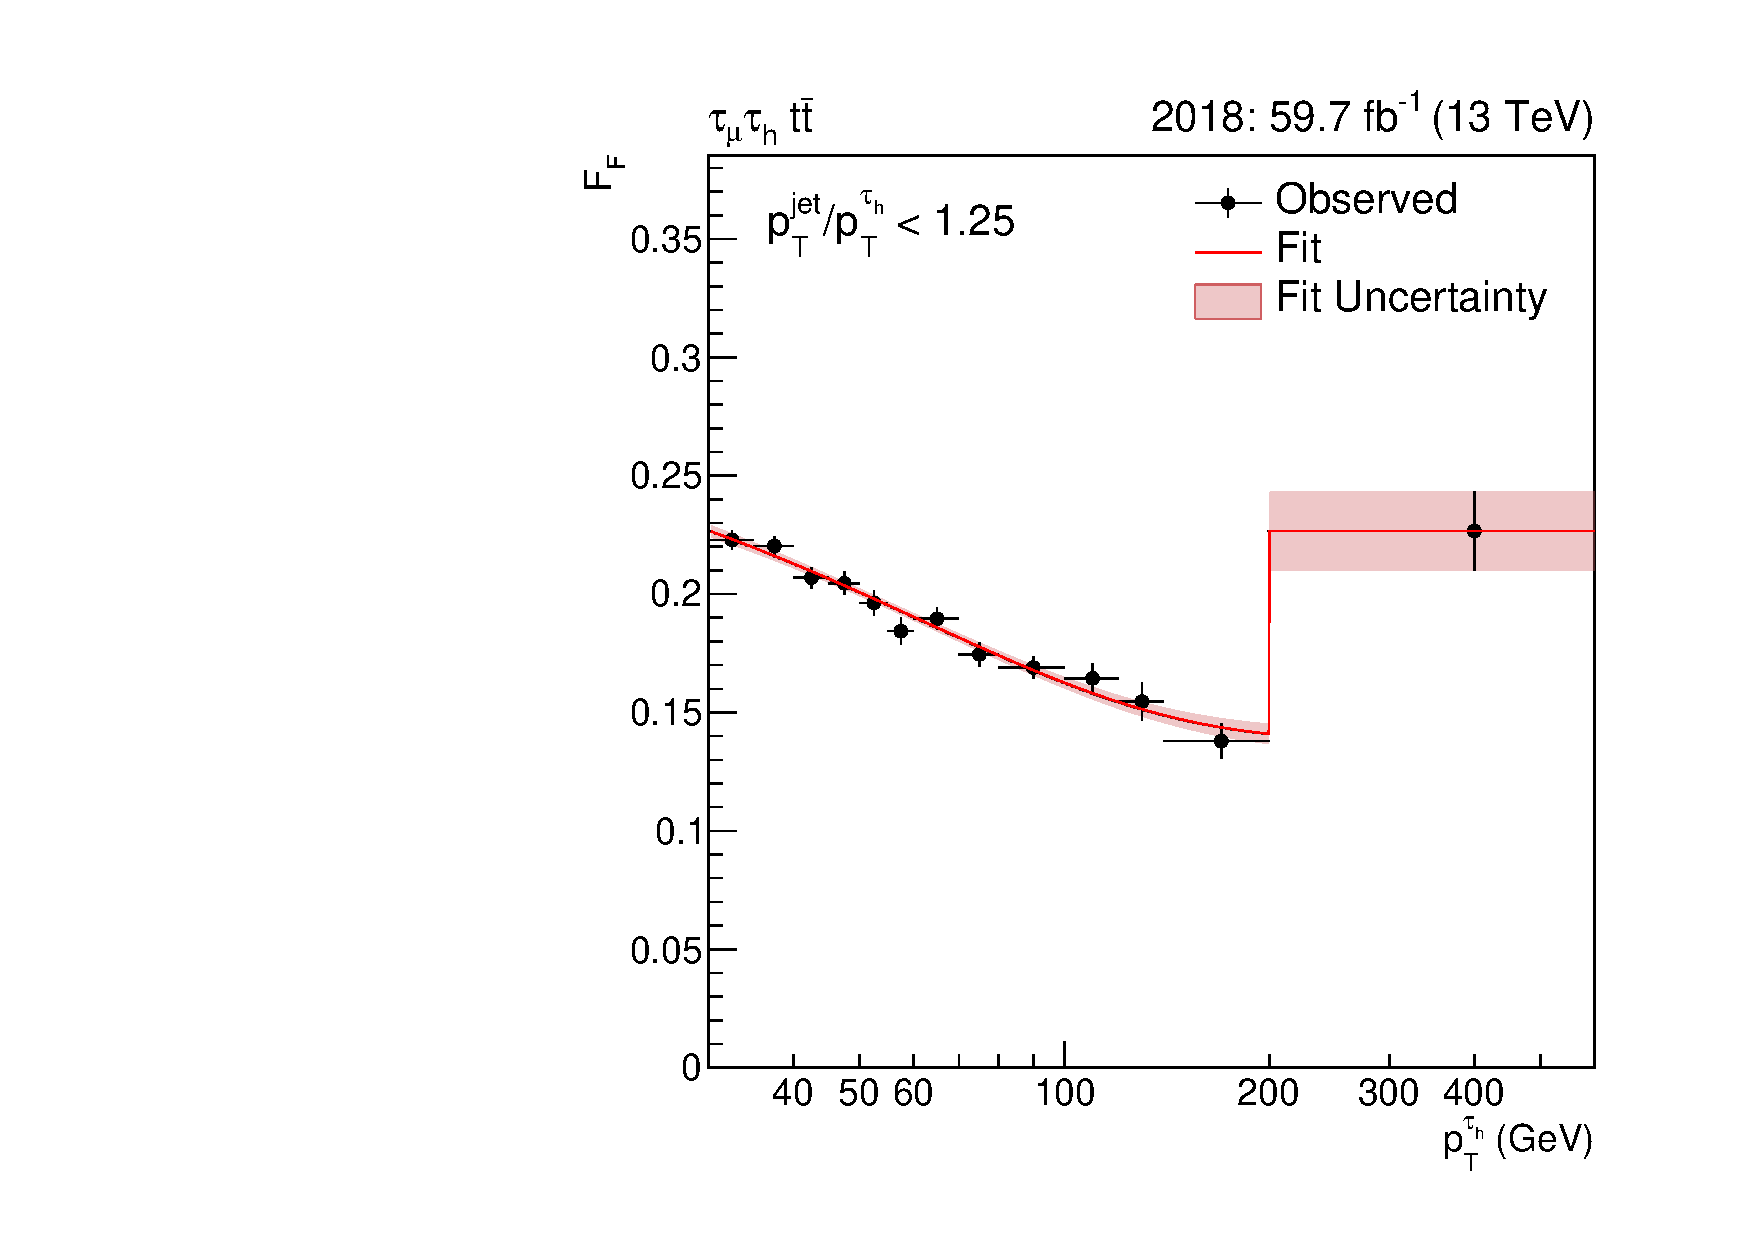
\includegraphics[width=.45\textwidth]{\PhDthesisdir/plots_and_images/from_CMS-NOTE-2020-218/ff_fit_jet_pt_low_inclusive_pt_2_ff_ttbar_mc_mt_2018.tex}}

\caption[Ajustements de $\FF_W$ et $\FF_t$ dans le canal \mu\tauh\ en 2018.]{Ajustements de $\FF_W$ et $\FF_t$ dans le canal \mu\tauh\ en 2018~\cite{CMS-NOTE-2020-218}.}
\label{fig-chapter-HTT_analysis-section-bg_estimation-FF_method-WJ-ttbar}
\end{figure}
\subsubsection{Corrections résiduelles}
Afin de valider les \fakefactors\ obtenus, ces derniers sont appliqués aux DRs pour les événements avec les mêmes points de fonctionnement de l'algorithme \DEEPTAU.
Les prédictions obtenues par les \fakefactors\ doivent alors correspondre aux observations brutes, \ie\ sans leur application.
Les écarts résiduels donnent la correction à appliquer, paramétrisée en fonction:
\begin{itemize}
\item du nombre de jets \Nprebjets\ identifiés comme issus de quarks~\quarkb, \Nbjets;
\item de l'impulsion transverse du lepton $\ell\in\set{\ele,\mu}$ pour les canaux semi-leptoniques, $\pT^{\ell}$;
\item de l'isolation du lepton $\ell\in\set{\ele,\mu}$ pour les canaux semi-leptoniques, $I^{\ell}$;
\item de la quantité d'énergie transverse manquante alignée avec le \tauh\ pour les événements QCD, $C_Q$,
\begin{equation}
C_Q = \frac{\MET}{\pT^{\tauh}} \cos(\Delta\phi(\vMET, \vpT^{\tauh}))
\mend[;]
\label{eq-FF_CQ_def}
\end{equation}
\item de la quantité d'énergie transverse manquante alignée avec le \tauh\ pour les événements \Wjets, $C_W$,
\begin{equation}
C_W = \frac{\norm{\vMET + \vpT^{\ell}}}{\pT^{\tauh}} \cos(\Delta\phi(\vMET + \vpT^{\ell}, \vpT^{\tauh}))
\mend[,]
\label{eq-FF_CW_def}
\end{equation}
dont la définition est semblable à celle de $C_Q$ mais où $\vMET$ est remplacé par $\vMET + \vpT^{\ell}$ afin de prendre en compte la contribution à \MET\ du neutrino issu de la désintégration du boson \Wboson.
Il est ici considéré comme dos-à-dos avec $\ell$, ce qui n'est strictement vrai que pour un \Wboson\ au repos.
\end{itemize}
%Les distributions de diverses variables, observées et prédites par les \fakefactors, doivent correspondre les unes aux autres.
%Les écarts résiduels entre observations et prédictions sont corrigées pour les variables qui n'ont pas encore été utilisées pour paramétriser les \fakefactors.
%\MET\ et $\pT^{\ell}$ observées et prédites par les \fakefactors\ doivent correspondre les unes aux autres.
%Les différences résiduelles sont alors corrigées.
%\par
%Les valeurs de \MET\ utilisées pour $\FF_Q$ sont corrigées en fonction de $C_Q$, définie équation~\eqref{eq-FF_CQ_def}.
%La correction est obtenue par un ajustement polynomial aux différences observées pour $\Nprebjets=0$ et $\Nprebjets\geq1$.
%Dans le cas de $\FF_W$ et $\FF_t$, les  valeurs de \MET\ utilisées sont corrigées en fonction de $C_W$, définie équation~\eqref{eq-FF_CW_def}.
%Un ajustement polynomial est réalisé dans les cas $\Nprebjets=0$ et $\Nprebjets\geq1$ pour $\FF_W$ et dans le cas général ($\Nprebjets\geq0$) pour $\FF_t$.
%\par
%Une fois les  valeurs de \MET\ corrigées, les distributions de $\pT^{\ell}$ le sont également pour $\FF_W$ et $\FF_t$.
Deux de ces corrections résiduelles obtenues sur le canal \mu\tauh\ en 2018 sont illustrées sur la figure~\ref{fig-chapter-HTT_analysis-section-bg_estimation-FF_method-closure}.
\begin{figure}[h]
\centering

\subcaptionbox{En fonction de $I_\mathrm{rel}^{(\mu)}$ pour $\FF_Q$.\label{subfig-chapter-HTT_analysis-section-bg_estimation-FF_method-closure-Q}}[.45\textwidth]
{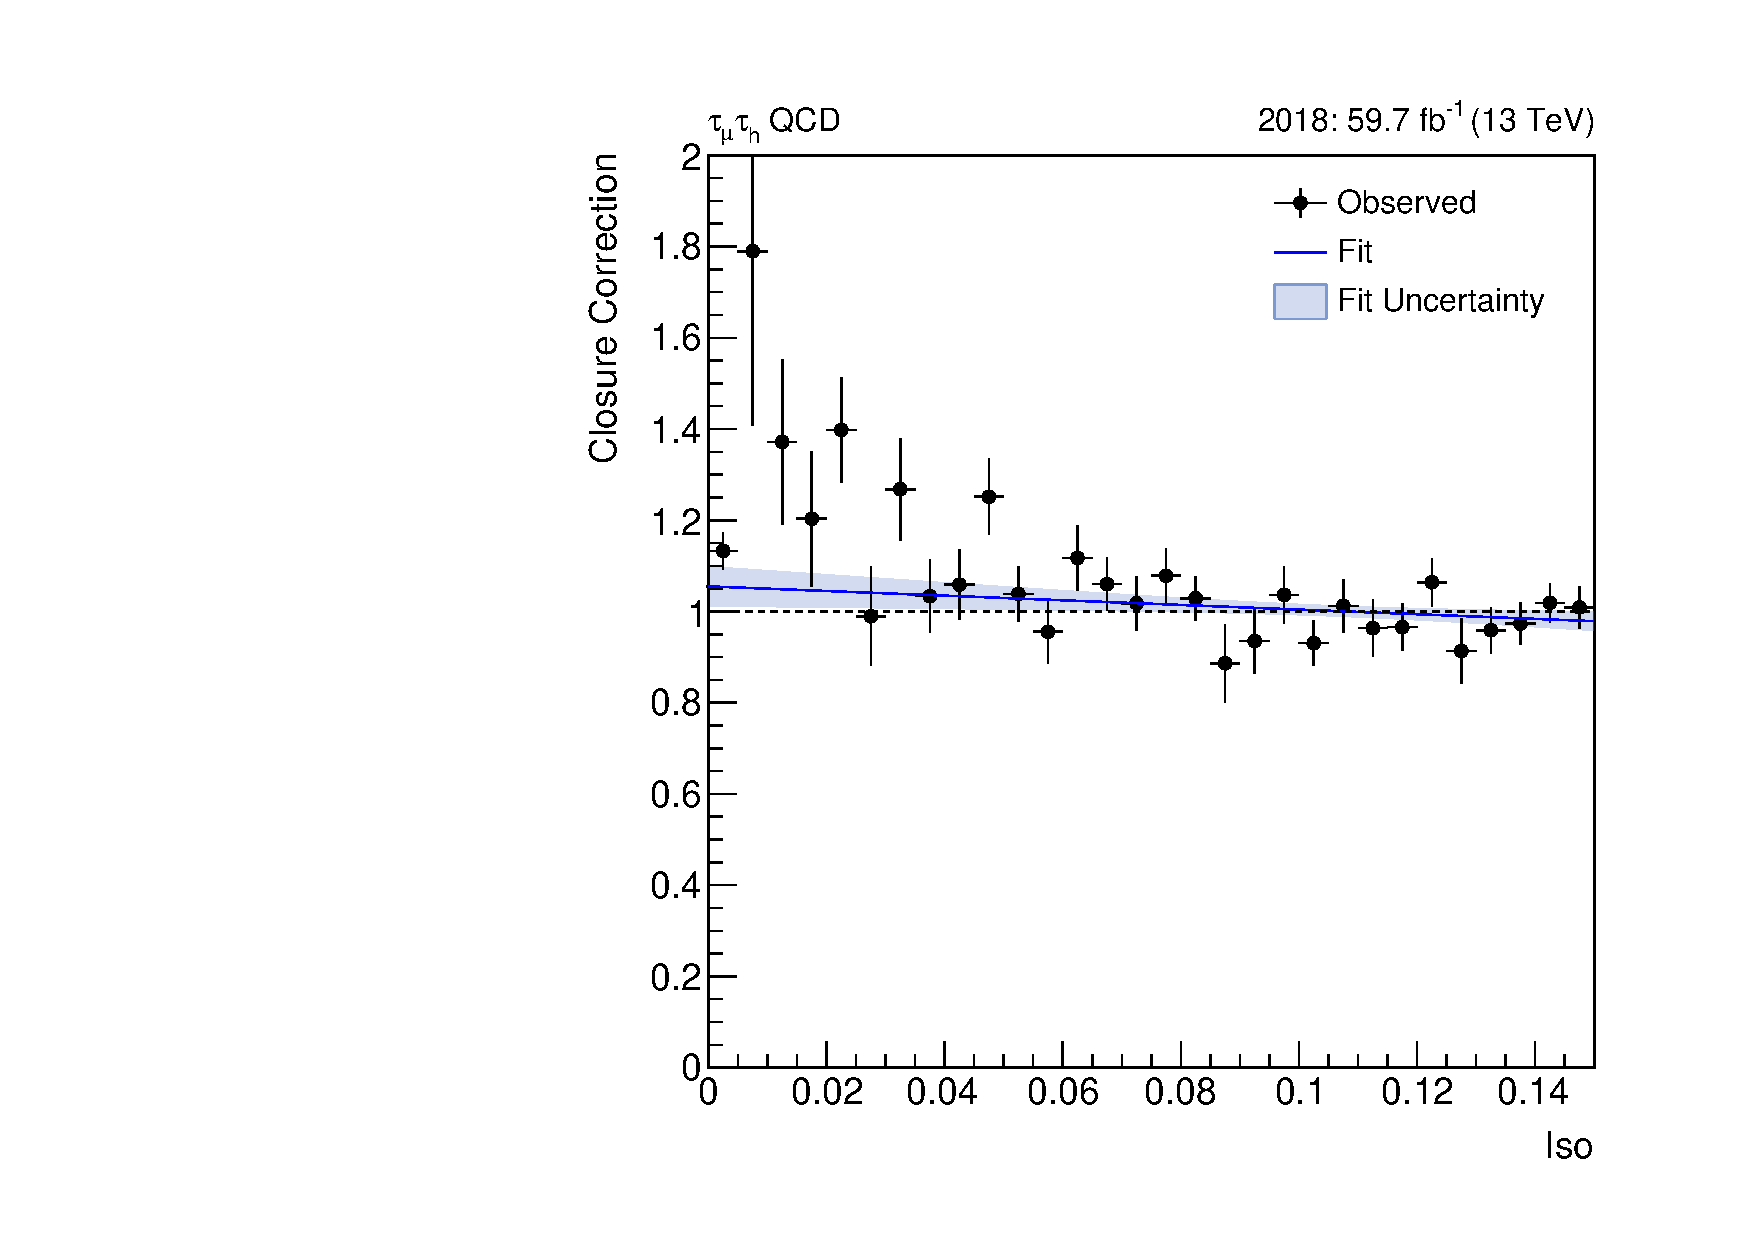
\includegraphics[width=.45\textwidth]{\PhDthesisdir/plots_and_images/from_CMS-NOTE-2020-218/ff_closure_iso_inclusive_closure_qcd_alt_mt_2018.tex}}
\hfill
\subcaptionbox{En fonction de $C_W$ pour $\FF_W$\label{subfig-chapter-HTT_analysis-section-bg_estimation-FF_method-closure-W}}[.45\textwidth]
{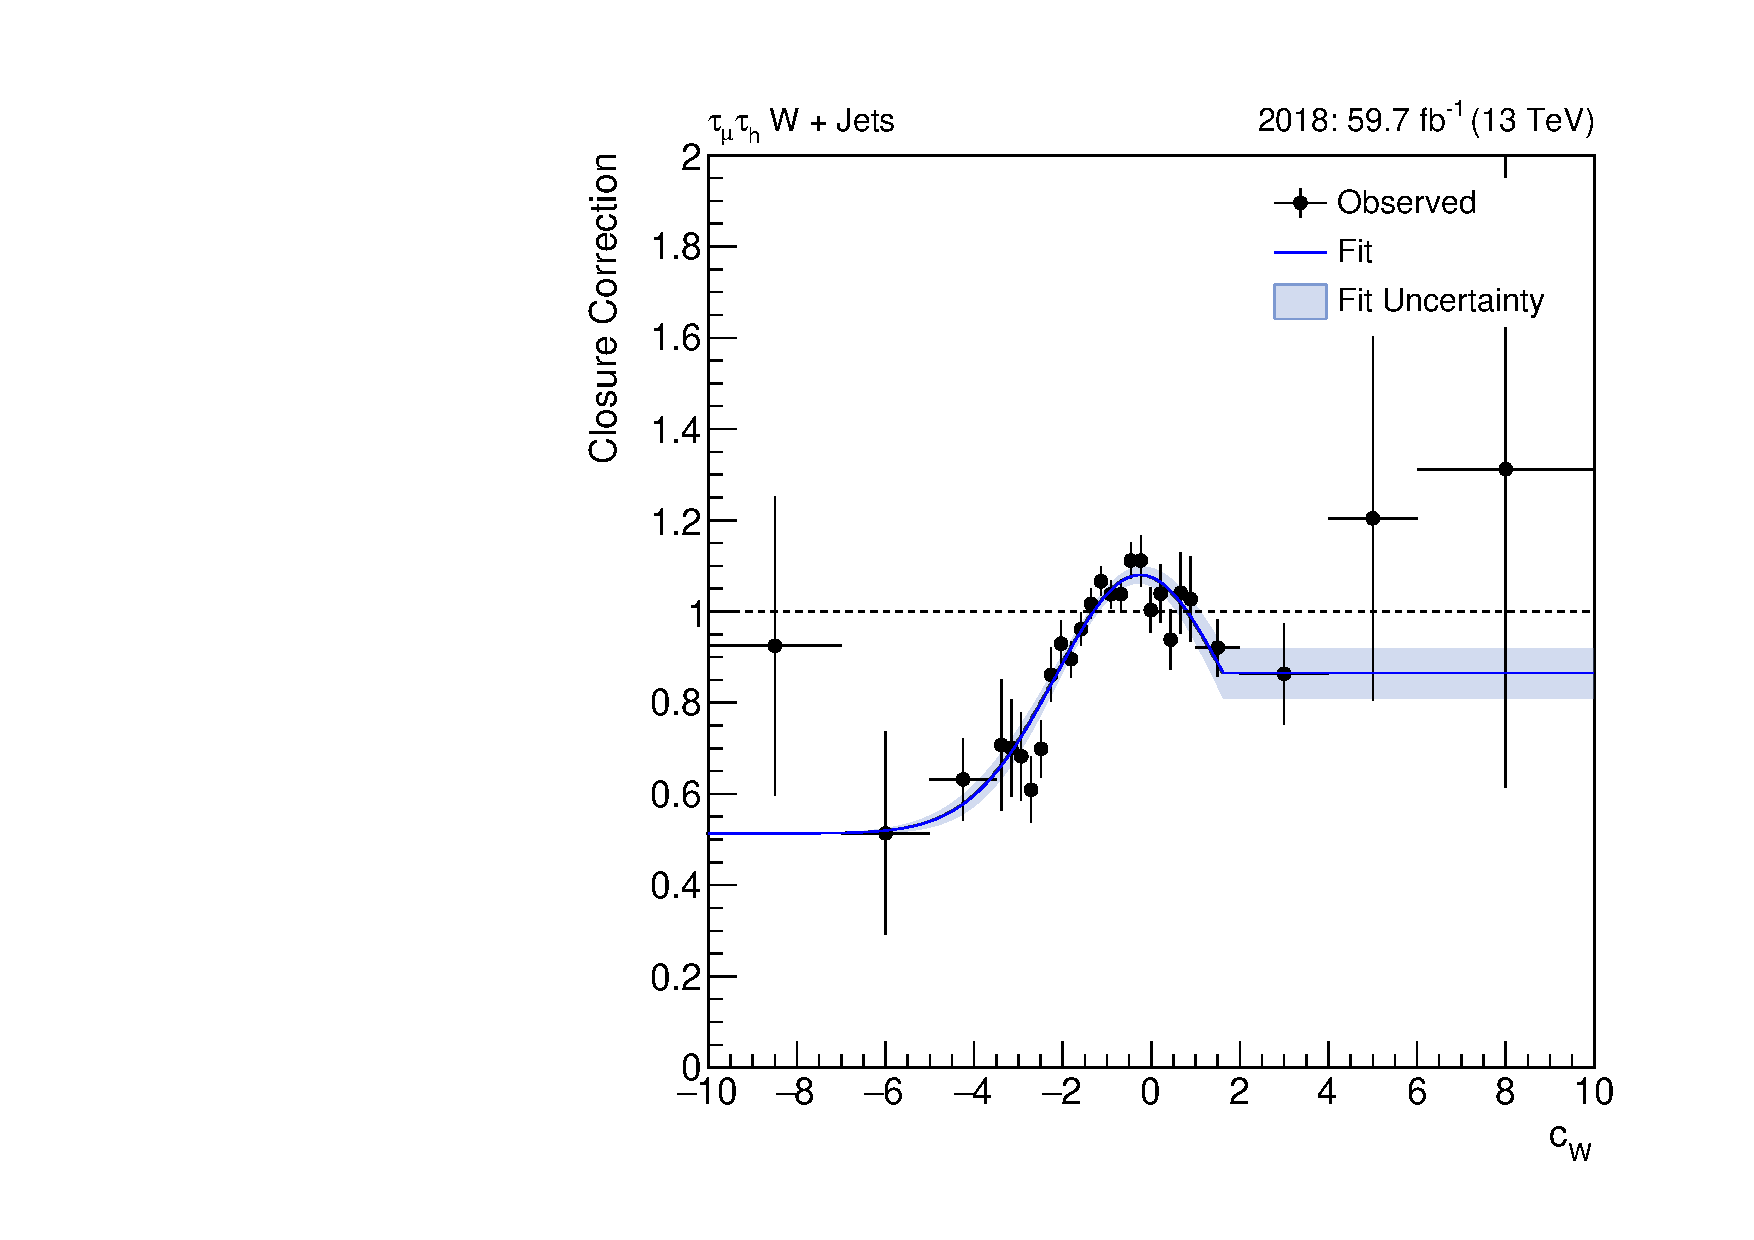
\includegraphics[width=.45\textwidth]{\PhDthesisdir/plots_and_images/from_CMS-NOTE-2020-218/ff_closure_met_1jet_closure_wjets_mt_2018.tex}}

\caption[Corrections résiduelles des \fakefactors\ dans le canal \mu\tauh\ en 2018.]{Corrections résiduelles des \fakefactors\ dans le canal \mu\tauh\ en 2018~\cite{CMS-NOTE-2020-218}.}
\label{fig-chapter-HTT_analysis-section-bg_estimation-FF_method-closure}
\end{figure}
\par
L'amélioration de la description des données ainsi obtenue grâce aux \fakefactors\ est visible sur la figure~\ref{fig-chapter-HTT_analysis-section-bg_estimation-FF_method-2018et_mT1_illustration}, où les distributions de la masse transverse de l'électron dans le canal \ele\tauh\ dans les données et dans l'estimation du bruit de fond sans et avec cette méthode sont tracées à titre d'illustration.
Outre un meilleur accord entre observations et estimation du bruit de fond, l'incertitude statistique est également réduite.
\begin{figure}[h]
\centering

\subcaptionbox{Sans \fakefactors.}[.475\textwidth]
{\plotHTTcontrol{2018}{emb_classic}{et}{mt_1_puppi}}
\hfill
\subcaptionbox{Avec \fakefactors.}[.475\textwidth]
{\plotHTTcontrol{2018}{emb_ff}{et}{mt_1_puppi}}

\caption{Distributions de la masse transverse de l'électron pour le canal \ele\tauh\ en 2018.}
\label{fig-chapter-HTT_analysis-section-bg_estimation-FF_method-2018et_mT1_illustration}
\end{figure}
\subsection{Estimation du bruit de fond QCD dans le canal \ele\mu}\label{chapter-HTT_analysis-section-bg_estimation-QCD-SS}
Dans le cas du canal \ele\mu, le bruit de fond QCD contribue à la sélection des événements lorsqu'au moins un jet est identifié à tort comme un électron ou un muon.
Une estimation de cette contribution est réalisée à partir des données réelles en suivant le principe de la méthode \og ABCD \fg.
\begin{wrapfigure}{R}{7.25cm}
\centering
\begin{tikzpicture}[scale=.8]
\draw (-2,0)--(2,0);
\draw (0,-2)--(0,2);
\draw (-1,1) node {A = SR};
\draw (1,1) node {C};
\draw (-1,-1) node {B = AR};
\draw (1,-1) node {D};
\draw (-2,1) node [left] {OS};
\draw (-2,-1) node [left] {SS};
\draw (-2,2) node [above left] {\mu:};
\draw (-1,2) node [above] {isolé\vphantom{\mu:}};
\draw (1,2) node [above] {anti-isolé\vphantom{\mu:}};
\end{tikzpicture}
\caption[Régions A, B, C et D utilisées pour estimer le bruit de fond QCD.]{Définition schématique des régions A, B, C et D pour l'estimation du bruit de fond QCD.}
\label{fig-ABCD_regions_schem}
\end{wrapfigure}
\par
Quatre régions pouvant se résumer schématiquement comme illustré sur la figure~\ref{fig-ABCD_regions_schem} sont définies:
\begin{description}
\item[A] région de signal (SR), définie dans la section~\ref{chapter-HTT_analysis-section-selection};
\item[B] définie comme la SR mais avec les charges électriques de l'électron et du muon de même signe (SS, \emph{Same Signs}) et non de signes opposés (OS, \emph{Opposite Signs}) comme dans la SR;
\item[C] définie comme la SR mais avec un muon \og anti-isolé \fg{}, \ie\ que la coupure sur son isolation est inversée, $\num{0.2}\leq I_\text{rel}^{\mu} < \num{0.5}$ au lieu de $I_\text{rel}^{\mu} < \num{0.2}$;
\item[D] définie comme la SR mais avec muon anti-isolé et SS.
\end{description}
Les hypothèses d'application de cette méthode sont:
\begin{itemize}
\item la forme de la distribution de la variable $v$ issue du bruit de fond QCD est identique dans la région A à déterminer et dans la région B connue;
\item le rapport du nombre d'événements entre A et B est le même qu'entre C et D.
\end{itemize}
Les contributions des bruits de fond autres que QCD aux régions B, C et D sont soustraits à partir de données simulées.
\par
La méthode ABCD permet alors d'obtenir le bruit de fond QCD dans la région de signal A selon ce qui s'assimile à un produit en croix,
\begin{equation}
A = B \times \frac{C}{D} \Leftrightarrow h_v^\text{A} = h_v^\text{B} \times \frac{\int h_v^\text{C}}{\int h_v^\text{D}}
\end{equation}
où $h_v^\text{X}$ correspond à la distribution de la variable $v$ dans la région X et $\int h_v^\text{X}$ à son intégrale, \ie\ la quantité d'événements (indépendante de $v$).
La région B est ainsi également nommée région d'application (AR, \emph{Application Region}) du facteur $C/D$.
\par
Afin d'augmenter la quantité d'événements exploités, et donc de réduire l'incertitude statistique, la coupure sur \Dzeta\ n'est pas appliquée dans les régions C et D.
Cependant, un facteur $C/D$ global donne une estimation trop peu précise~\cite{CMS-PAS-HIG-18-032} car l'hypothèse d'indépendance de la forme de la distribution n'est pas vérifiée.
Afin de corriger cet effet, le facteur $C/D$ est déterminé en fonction de:
\begin{itemize}
\item la distance entre l'électron et le muon dans le plan $(\eta,\phi)$, $\Delta R$;
\item le nombre de jets \Njets;
\item l'impulsion transverse de l'électron, $\pT^{\ele}$;
\item l'impulsion transverse du muon, $\pT^{\mu}$;
\end{itemize}
La dépendance en $\Delta R$ est majoritairement due à la contribution \quarkb\antiquarkb\ au bruit de fond QCD.
Elle est modélisée par un polynôme de degré 2.
\par
Afin de corriger le biais introduit par le changement de critère d'isolation du muon, le facteur $C/D$ est également déterminé dans les cas de figure suivants:
\begin{itemize}
\item électron anti-isolé ($\num{0.15}\leq I_\text{rel}^{\ele} < \num{0.5}$ au lieu de $I_\text{rel}^{\ele} < \num{0.15}$) et muon isolé;
\item électron et muon anti-isolés.
\end{itemize}
Le rapport de ces facteurs donne la correction relative au passage des muons isolés à anti-isolés.
\subsection{Estimations à partir de simulations}\label{chapter-HTT_analysis-section-bg_estimation-MC}

% HIG 17 20
All other backgrounds are taken from simulation.
%For this purpose the simulated events are
%corrected to match the pileup distribution observed in data. Further corrections are derived
%to account for residual differences in the efficiency of the selected trigger paths, for the differ-
%ences in the electron and muon tracking efficiency and in the efficiency of the identification
%and isolation requirements for electrons and muons.